\documentclass[twoside]{book}

% Packages required by doxygen
\usepackage{fixltx2e}
\usepackage{calc}
\usepackage{doxygen}
\usepackage[export]{adjustbox} % also loads graphicx
\usepackage{graphicx}
\usepackage[utf8]{inputenc}
\usepackage{makeidx}
\usepackage{multicol}
\usepackage{multirow}
\PassOptionsToPackage{warn}{textcomp}
\usepackage{textcomp}
\usepackage[nointegrals]{wasysym}
\usepackage[table]{xcolor}

% Font selection
\usepackage[T1]{fontenc}
\usepackage[scaled=.90]{helvet}
\usepackage{courier}
\usepackage{amssymb}
\usepackage{sectsty}
\renewcommand{\familydefault}{\sfdefault}
\allsectionsfont{%
  \fontseries{bc}\selectfont%
  \color{darkgray}%
}
\renewcommand{\DoxyLabelFont}{%
  \fontseries{bc}\selectfont%
  \color{darkgray}%
}
\newcommand{\+}{\discretionary{\mbox{\scriptsize$\hookleftarrow$}}{}{}}

% Page & text layout
\usepackage{geometry}
\geometry{%
  a4paper,%
  top=2.5cm,%
  bottom=2.5cm,%
  left=2.5cm,%
  right=2.5cm%
}
\tolerance=750
\hfuzz=15pt
\hbadness=750
\setlength{\emergencystretch}{15pt}
\setlength{\parindent}{0cm}
\setlength{\parskip}{3ex plus 2ex minus 2ex}
\makeatletter
\renewcommand{\paragraph}{%
  \@startsection{paragraph}{4}{0ex}{-1.0ex}{1.0ex}{%
    \normalfont\normalsize\bfseries\SS@parafont%
  }%
}
\renewcommand{\subparagraph}{%
  \@startsection{subparagraph}{5}{0ex}{-1.0ex}{1.0ex}{%
    \normalfont\normalsize\bfseries\SS@subparafont%
  }%
}
\makeatother

% Headers & footers
\usepackage{fancyhdr}
\pagestyle{fancyplain}
\fancyhead[LE]{\fancyplain{}{\bfseries\thepage}}
\fancyhead[CE]{\fancyplain{}{}}
\fancyhead[RE]{\fancyplain{}{\bfseries\leftmark}}
\fancyhead[LO]{\fancyplain{}{\bfseries\rightmark}}
\fancyhead[CO]{\fancyplain{}{}}
\fancyhead[RO]{\fancyplain{}{\bfseries\thepage}}
\fancyfoot[LE]{\fancyplain{}{}}
\fancyfoot[CE]{\fancyplain{}{}}
\fancyfoot[RE]{\fancyplain{}{\bfseries\scriptsize Generated by Doxygen }}
\fancyfoot[LO]{\fancyplain{}{\bfseries\scriptsize Generated by Doxygen }}
\fancyfoot[CO]{\fancyplain{}{}}
\fancyfoot[RO]{\fancyplain{}{}}
\renewcommand{\footrulewidth}{0.4pt}
\renewcommand{\chaptermark}[1]{%
  \markboth{#1}{}%
}
\renewcommand{\sectionmark}[1]{%
  \markright{\thesection\ #1}%
}

% Indices & bibliography
\usepackage{natbib}
\usepackage[titles]{tocloft}
\setcounter{tocdepth}{3}
\setcounter{secnumdepth}{5}
\makeindex

% Hyperlinks (required, but should be loaded last)
\usepackage{ifpdf}
\ifpdf
  \usepackage[pdftex,pagebackref=true]{hyperref}
\else
  \usepackage[ps2pdf,pagebackref=true]{hyperref}
\fi
\hypersetup{%
  colorlinks=true,%
  linkcolor=blue,%
  citecolor=blue,%
  unicode%
}

% Custom commands
\newcommand{\clearemptydoublepage}{%
  \newpage{\pagestyle{empty}\cleardoublepage}%
}

\usepackage{caption}
\captionsetup{labelsep=space,justification=centering,font={bf},singlelinecheck=off,skip=4pt,position=top}

%===== C O N T E N T S =====

\begin{document}

% Titlepage & ToC
\hypersetup{pageanchor=false,
             bookmarksnumbered=true,
             pdfencoding=unicode
            }
\pagenumbering{alph}
\begin{titlepage}
\vspace*{7cm}
\begin{center}%
{\Large P\+O\+SL \\[1ex]\large 1.\+0 }\\
\vspace*{1cm}
{\large Generated by Doxygen 1.8.13}\\
\end{center}
\end{titlepage}
\clearemptydoublepage
\pagenumbering{roman}
\tableofcontents
\clearemptydoublepage
\pagenumbering{arabic}
\hypersetup{pageanchor=true}

%--- Begin generated contents ---
\chapter{P\+O\+SL}
\label{index}\hypertarget{index}{}A parallel Oriented Solver Language

\subsection*{Introduction }

The multi-\/core technology and massive parallel architectures are nowadays more accessible for a broad public through hardware like the Xeon Phi or G\+PU cards. This architecture strategy has been commonly adopted by processor manufacturers to stick with Moore’s law. However, this new architecture implies new ways of designing and implementing algorithms to exploit their full potential. This is in particular true for constraint-\/based solvers dealing with combinatorial optimization problems.

Furthermore, the developing time needed to code parallel solvers is often underestimated. In fact, conceiving efficient algorithms to solve certain problems takes a considerable amount of time. In this thesis we present \hyperlink{namespacePOSL}{P\+O\+SL}, a Parallel-\/\+Oriented Solver Language for building solvers based on meta-\/heuristic in order to solve Constraint Satisfaction Problems (C\+SP) in parallel. The main goal of this thesis is to obtain a system with which solvers can be easily built, reducing therefore their development effort by proposing a mechanism for code reusing between solvers. It also provides a mechanism to implement solver-\/independent communication strategies. We also present a detailed analysis of the results obtained when solving some C\+S\+Ps. The goal is not to outperform the state of the art solvers in terms of efficiency, but to show that it is possible to rapidly prototype with \hyperlink{namespacePOSL}{P\+O\+SL} in order to experiment different communication strategies. 
\chapter{Namespace Index}
\section{Namespace List}
Here is a list of all documented namespaces with brief descriptions\+:\begin{DoxyCompactList}
\item\contentsline{section}{\hyperlink{namespacePOSL}{P\+O\+SL} }{\pageref{namespacePOSL}}{}
\item\contentsline{section}{\hyperlink{namespacePOSL_1_1Benchmarks}{P\+O\+S\+L.\+Benchmarks} \\*Class to represent the absolute cost stratategy of Social Golgers Problem }{\pageref{namespacePOSL_1_1Benchmarks}}{}
\item\contentsline{section}{\hyperlink{namespacePOSL_1_1Data}{P\+O\+S\+L.\+Data} \\*(Abstract) Class to represent all types of I/O in \hyperlink{namespacePOSL}{P\+O\+SL} }{\pageref{namespacePOSL_1_1Data}}{}
\item\contentsline{section}{\hyperlink{namespacePOSL_1_1Solver}{P\+O\+S\+L.\+Solver} }{\pageref{namespacePOSL_1_1Solver}}{}
\item\contentsline{section}{\hyperlink{namespacePOSL_1_1Tools}{P\+O\+S\+L.\+Tools} \\*Interface to represent the a class that can projec the cost of a variable }{\pageref{namespacePOSL_1_1Tools}}{}
\end{DoxyCompactList}

\chapter{Hierarchical Index}
\section{Class Hierarchy}
This inheritance list is sorted roughly, but not completely, alphabetically\+:\begin{DoxyCompactList}
\item \contentsline{section}{P\+O\+S\+L.\+Benchmarks.\+Benchmark}{\pageref{classPOSL_1_1Benchmarks_1_1Benchmark}}{}
\begin{DoxyCompactList}
\item \contentsline{section}{P\+O\+S\+L.\+Benchmarks.\+Golfers}{\pageref{classPOSL_1_1Benchmarks_1_1Golfers}}{}
\end{DoxyCompactList}
\item \contentsline{section}{P\+O\+S\+L.\+Data.\+Computation\+Data}{\pageref{classPOSL_1_1Data_1_1ComputationData}}{}
\begin{DoxyCompactList}
\item \contentsline{section}{P\+O\+S\+L.\+Data.\+Decision\+Pair}{\pageref{classPOSL_1_1Data_1_1DecisionPair}}{}
\item \contentsline{section}{P\+O\+S\+L.\+Data.\+Neighborhood}{\pageref{classPOSL_1_1Data_1_1Neighborhood}}{}
\item \contentsline{section}{P\+O\+S\+L.\+Data.\+Solution}{\pageref{classPOSL_1_1Data_1_1Solution}}{}
\end{DoxyCompactList}
\item \contentsline{section}{P\+O\+S\+L.\+Tools.\+Connection\+Matrix}{\pageref{classPOSL_1_1Tools_1_1ConnectionMatrix}}{}
\item \contentsline{section}{P\+O\+S\+L.\+Domain}{\pageref{classPOSL_1_1Domain}}{}
\begin{DoxyCompactList}
\item \contentsline{section}{P\+O\+S\+L.\+Data.\+Uniform\+Domain}{\pageref{classPOSL_1_1Data_1_1UniformDomain}}{}
\end{DoxyCompactList}
\item \contentsline{section}{P\+O\+S\+L.\+Benchmarks.\+I\+Cost\+Strategy}{\pageref{interfacePOSL_1_1Benchmarks_1_1ICostStrategy}}{}
\begin{DoxyCompactList}
\item \contentsline{section}{P\+O\+S\+L.\+Benchmarks.\+Golfers\+Long\+Int\+Cost\+Strategy}{\pageref{classPOSL_1_1Benchmarks_1_1GolfersLongIntCostStrategy}}{}
\end{DoxyCompactList}
\item \contentsline{section}{P\+O\+S\+L.\+Data.\+I\+Dynamic\+Neighborhood}{\pageref{interfacePOSL_1_1Data_1_1IDynamicNeighborhood}}{}
\item \contentsline{section}{P\+O\+S\+L.\+Data.\+I\+P\+O\+S\+L\+\_\+\+Iterator}{\pageref{interfacePOSL_1_1Data_1_1IPOSL__Iterator}}{}
\begin{DoxyCompactList}
\item \contentsline{section}{P\+O\+S\+L.\+Data.\+Elements\+Change\+Iterator}{\pageref{classPOSL_1_1Data_1_1ElementsChangeIterator}}{}
\end{DoxyCompactList}
\item \contentsline{section}{P\+O\+S\+L.\+Benchmarks.\+I\+Projectable\+Cost}{\pageref{interfacePOSL_1_1Benchmarks_1_1IProjectableCost}}{}
\item \contentsline{section}{P\+O\+S\+L.\+Benchmarks.\+I\+Relative\+Cost\+Strategy}{\pageref{interfacePOSL_1_1Benchmarks_1_1IRelativeCostStrategy}}{}
\begin{DoxyCompactList}
\item \contentsline{section}{P\+O\+S\+L.\+Benchmarks.\+Golfers\+Relative\+Cost\+Strategy}{\pageref{classPOSL_1_1Benchmarks_1_1GolfersRelativeCostStrategy}}{}
\end{DoxyCompactList}
\item \contentsline{section}{P\+O\+S\+L.\+Benchmarks.\+I\+Reseteable}{\pageref{interfacePOSL_1_1Benchmarks_1_1IReseteable}}{}
\item \contentsline{section}{P\+O\+S\+L.\+Benchmarks.\+I\+Show\+Strategy}{\pageref{interfacePOSL_1_1Benchmarks_1_1IShowStrategy}}{}
\begin{DoxyCompactList}
\item \contentsline{section}{P\+O\+S\+L.\+Benchmarks.\+Golfers\+Default\+Show\+Strategy}{\pageref{classPOSL_1_1Benchmarks_1_1GolfersDefaultShowStrategy}}{}
\end{DoxyCompactList}
\item \contentsline{section}{P\+O\+S\+L.\+Benchmarks.\+I\+Sickest\+Variable\+Strategy}{\pageref{interfacePOSL_1_1Benchmarks_1_1ISickestVariableStrategy}}{}
\item \contentsline{section}{P\+O\+S\+L.\+Tools.\+Long\+Int}{\pageref{classPOSL_1_1Tools_1_1LongInt}}{}
\item \contentsline{section}{P\+O\+S\+L.\+Tools.\+Merged\+Long\+Int}{\pageref{classPOSL_1_1Tools_1_1MergedLongInt}}{}
\item \contentsline{section}{P\+O\+S\+L.\+Tools.\+Posl\+Tools}{\pageref{classPOSL_1_1Tools_1_1PoslTools}}{}
\item \contentsline{section}{P\+O\+S\+L.\+Solver.\+P\+SP}{\pageref{classPOSL_1_1Solver_1_1PSP}}{}
\item \contentsline{section}{P\+O\+S\+L.\+Tools.\+Random\+Generator}{\pageref{classPOSL_1_1Tools_1_1RandomGenerator}}{}
\item \contentsline{section}{P\+O\+S\+L.\+Tools.\+T\+\_\+\+Changes}{\pageref{structPOSL_1_1Tools_1_1T__Changes}}{}
\end{DoxyCompactList}

\chapter{Class Index}
\section{Class List}
Here are the classes, structs, unions and interfaces with brief descriptions\+:\begin{DoxyCompactList}
\item\contentsline{section}{\hyperlink{classPOSL_1_1Benchmarks_1_1Benchmark}{P\+O\+S\+L.\+Benchmarks.\+Benchmark} \\*(Abstract) Class to represent an instance of a problem }{\pageref{classPOSL_1_1Benchmarks_1_1Benchmark}}{}
\item\contentsline{section}{\hyperlink{classPOSL_1_1Data_1_1ComputationData}{P\+O\+S\+L.\+Data.\+Computation\+Data} \\*(Abstract) Class to represent all types of I/O in \hyperlink{namespacePOSL}{P\+O\+SL} }{\pageref{classPOSL_1_1Data_1_1ComputationData}}{}
\item\contentsline{section}{\hyperlink{classPOSL_1_1Tools_1_1ConnectionMatrix}{P\+O\+S\+L.\+Tools.\+Connection\+Matrix} }{\pageref{classPOSL_1_1Tools_1_1ConnectionMatrix}}{}
\item\contentsline{section}{\hyperlink{classPOSL_1_1Data_1_1DecisionPair}{P\+O\+S\+L.\+Data.\+Decision\+Pair} \\*Class to represent a couple of solutions (current and new found) }{\pageref{classPOSL_1_1Data_1_1DecisionPair}}{}
\item\contentsline{section}{\hyperlink{classPOSL_1_1Domain}{P\+O\+S\+L.\+Domain} }{\pageref{classPOSL_1_1Domain}}{}
\item\contentsline{section}{\hyperlink{classPOSL_1_1Data_1_1ElementsChangeIterator}{P\+O\+S\+L.\+Data.\+Elements\+Change\+Iterator} }{\pageref{classPOSL_1_1Data_1_1ElementsChangeIterator}}{}
\item\contentsline{section}{\hyperlink{classPOSL_1_1Benchmarks_1_1Golfers}{P\+O\+S\+L.\+Benchmarks.\+Golfers} \\*Class to represent an instance of a \hyperlink{classPOSL_1_1Benchmarks_1_1Golfers}{Golfers} Problems }{\pageref{classPOSL_1_1Benchmarks_1_1Golfers}}{}
\item\contentsline{section}{\hyperlink{classPOSL_1_1Benchmarks_1_1GolfersDefaultShowStrategy}{P\+O\+S\+L.\+Benchmarks.\+Golfers\+Default\+Show\+Strategy} \\*Class to represent the way Social \hyperlink{classPOSL_1_1Benchmarks_1_1Golfers}{Golfers} problem shows its result (solution) }{\pageref{classPOSL_1_1Benchmarks_1_1GolfersDefaultShowStrategy}}{}
\item\contentsline{section}{\hyperlink{classPOSL_1_1Benchmarks_1_1GolfersLongIntCostStrategy}{P\+O\+S\+L.\+Benchmarks.\+Golfers\+Long\+Int\+Cost\+Strategy} \\*Class to represent the absolute cost stratategy of Social Golgers Problem }{\pageref{classPOSL_1_1Benchmarks_1_1GolfersLongIntCostStrategy}}{}
\item\contentsline{section}{\hyperlink{classPOSL_1_1Benchmarks_1_1GolfersRelativeCostStrategy}{P\+O\+S\+L.\+Benchmarks.\+Golfers\+Relative\+Cost\+Strategy} }{\pageref{classPOSL_1_1Benchmarks_1_1GolfersRelativeCostStrategy}}{}
\item\contentsline{section}{\hyperlink{interfacePOSL_1_1Benchmarks_1_1ICostStrategy}{P\+O\+S\+L.\+Benchmarks.\+I\+Cost\+Strategy} \\*Interface to represent an absolute solution cost strategy }{\pageref{interfacePOSL_1_1Benchmarks_1_1ICostStrategy}}{}
\item\contentsline{section}{\hyperlink{interfacePOSL_1_1Data_1_1IDynamicNeighborhood}{P\+O\+S\+L.\+Data.\+I\+Dynamic\+Neighborhood} }{\pageref{interfacePOSL_1_1Data_1_1IDynamicNeighborhood}}{}
\item\contentsline{section}{\hyperlink{interfacePOSL_1_1Data_1_1IPOSL__Iterator}{P\+O\+S\+L.\+Data.\+I\+P\+O\+S\+L\+\_\+\+Iterator} }{\pageref{interfacePOSL_1_1Data_1_1IPOSL__Iterator}}{}
\item\contentsline{section}{\hyperlink{interfacePOSL_1_1Benchmarks_1_1IProjectableCost}{P\+O\+S\+L.\+Benchmarks.\+I\+Projectable\+Cost} \\*Interface to represent the a class that can projec the cost of a variable }{\pageref{interfacePOSL_1_1Benchmarks_1_1IProjectableCost}}{}
\item\contentsline{section}{\hyperlink{interfacePOSL_1_1Benchmarks_1_1IRelativeCostStrategy}{P\+O\+S\+L.\+Benchmarks.\+I\+Relative\+Cost\+Strategy} \\*Interface to represent a relative solution cost strategy }{\pageref{interfacePOSL_1_1Benchmarks_1_1IRelativeCostStrategy}}{}
\item\contentsline{section}{\hyperlink{interfacePOSL_1_1Benchmarks_1_1IReseteable}{P\+O\+S\+L.\+Benchmarks.\+I\+Reseteable} \\*Interface to represent a relative solution cost strategy }{\pageref{interfacePOSL_1_1Benchmarks_1_1IReseteable}}{}
\item\contentsline{section}{\hyperlink{interfacePOSL_1_1Benchmarks_1_1IShowStrategy}{P\+O\+S\+L.\+Benchmarks.\+I\+Show\+Strategy} \\*Interface to represent the way a problem shows its result (solution) }{\pageref{interfacePOSL_1_1Benchmarks_1_1IShowStrategy}}{}
\item\contentsline{section}{\hyperlink{interfacePOSL_1_1Benchmarks_1_1ISickestVariableStrategy}{P\+O\+S\+L.\+Benchmarks.\+I\+Sickest\+Variable\+Strategy} \\*Interface to represent a strategy to compute the variable with the highest projected cost }{\pageref{interfacePOSL_1_1Benchmarks_1_1ISickestVariableStrategy}}{}
\item\contentsline{section}{\hyperlink{classPOSL_1_1Tools_1_1LongInt}{P\+O\+S\+L.\+Tools.\+Long\+Int} }{\pageref{classPOSL_1_1Tools_1_1LongInt}}{}
\item\contentsline{section}{\hyperlink{classPOSL_1_1Tools_1_1MergedLongInt}{P\+O\+S\+L.\+Tools.\+Merged\+Long\+Int} }{\pageref{classPOSL_1_1Tools_1_1MergedLongInt}}{}
\item\contentsline{section}{\hyperlink{classPOSL_1_1Data_1_1Neighborhood}{P\+O\+S\+L.\+Data.\+Neighborhood} \\*(Abstract) Class to represent a neighborhood of a configuration }{\pageref{classPOSL_1_1Data_1_1Neighborhood}}{}
\item\contentsline{section}{\hyperlink{classPOSL_1_1Tools_1_1PoslTools}{P\+O\+S\+L.\+Tools.\+Posl\+Tools} }{\pageref{classPOSL_1_1Tools_1_1PoslTools}}{}
\item\contentsline{section}{\hyperlink{classPOSL_1_1Solver_1_1PSP}{P\+O\+S\+L.\+Solver.\+P\+SP} }{\pageref{classPOSL_1_1Solver_1_1PSP}}{}
\item\contentsline{section}{\hyperlink{classPOSL_1_1Tools_1_1RandomGenerator}{P\+O\+S\+L.\+Tools.\+Random\+Generator} }{\pageref{classPOSL_1_1Tools_1_1RandomGenerator}}{}
\item\contentsline{section}{\hyperlink{classPOSL_1_1Data_1_1Solution}{P\+O\+S\+L.\+Data.\+Solution} }{\pageref{classPOSL_1_1Data_1_1Solution}}{}
\item\contentsline{section}{\hyperlink{structPOSL_1_1Tools_1_1T__Changes}{P\+O\+S\+L.\+Tools.\+T\+\_\+\+Changes} }{\pageref{structPOSL_1_1Tools_1_1T__Changes}}{}
\item\contentsline{section}{\hyperlink{classPOSL_1_1Data_1_1UniformDomain}{P\+O\+S\+L.\+Data.\+Uniform\+Domain} }{\pageref{classPOSL_1_1Data_1_1UniformDomain}}{}
\end{DoxyCompactList}

\chapter{Namespace Documentation}
\hypertarget{namespacePOSL}{}\section{P\+O\+SL Namespace Reference}
\label{namespacePOSL}\index{P\+O\+SL@{P\+O\+SL}}
\subsection*{Namespaces}
\begin{DoxyCompactItemize}
\item 
namespace \hyperlink{namespacePOSL_1_1Benchmarks}{Benchmarks}
\begin{DoxyCompactList}\small\item\em Class to represent the absolute cost stratategy of Social Golgers Problem. \end{DoxyCompactList}\item 
namespace \hyperlink{namespacePOSL_1_1Data}{Data}
\begin{DoxyCompactList}\small\item\em (Abstract) Class to represent all types of I/O in \hyperlink{namespacePOSL}{P\+O\+SL} \end{DoxyCompactList}\item 
namespace \hyperlink{namespacePOSL_1_1Tools}{Tools}
\begin{DoxyCompactList}\small\item\em Interface to represent the a class that can projec the cost of a variable. \end{DoxyCompactList}\end{DoxyCompactItemize}
\subsection*{Classes}
\begin{DoxyCompactItemize}
\item 
class \hyperlink{classPOSL_1_1Domain}{Domain}
\end{DoxyCompactItemize}

\hypertarget{namespacePOSL_1_1Benchmarks}{}\section{P\+O\+S\+L.\+Benchmarks Namespace Reference}
\label{namespacePOSL_1_1Benchmarks}\index{P\+O\+S\+L.\+Benchmarks@{P\+O\+S\+L.\+Benchmarks}}


Class to represent the absolute cost stratategy of Social Golgers Problem.  


\subsection*{Classes}
\begin{DoxyCompactItemize}
\item 
class \hyperlink{classPOSL_1_1Benchmarks_1_1Benchmark}{Benchmark}
\begin{DoxyCompactList}\small\item\em (Abstract) Class to represent an instance of a problem \end{DoxyCompactList}\item 
class \hyperlink{classPOSL_1_1Benchmarks_1_1Golfers}{Golfers}
\begin{DoxyCompactList}\small\item\em Class to represent an instance of a \hyperlink{classPOSL_1_1Benchmarks_1_1Golfers}{Golfers} Problems. \end{DoxyCompactList}\item 
class \hyperlink{classPOSL_1_1Benchmarks_1_1GolfersDefaultShowStrategy}{Golfers\+Default\+Show\+Strategy}
\begin{DoxyCompactList}\small\item\em Class to represent the way Social \hyperlink{classPOSL_1_1Benchmarks_1_1Golfers}{Golfers} problem shows its result (solution) \end{DoxyCompactList}\item 
class \hyperlink{classPOSL_1_1Benchmarks_1_1GolfersLongIntCostStrategy}{Golfers\+Long\+Int\+Cost\+Strategy}
\begin{DoxyCompactList}\small\item\em Class to represent the absolute cost stratategy of Social Golgers Problem. \end{DoxyCompactList}\item 
class \hyperlink{classPOSL_1_1Benchmarks_1_1GolfersRelativeCostStrategy}{Golfers\+Relative\+Cost\+Strategy}
\item 
class \hyperlink{interfacePOSL_1_1Benchmarks_1_1ICostStrategy}{I\+Cost\+Strategy}
\begin{DoxyCompactList}\small\item\em Interface to represent an absolute solution cost strategy. \end{DoxyCompactList}\item 
class \hyperlink{interfacePOSL_1_1Benchmarks_1_1IProjectableCost}{I\+Projectable\+Cost}
\begin{DoxyCompactList}\small\item\em Interface to represent the a class that can projec the cost of a variable. \end{DoxyCompactList}\item 
class \hyperlink{interfacePOSL_1_1Benchmarks_1_1IRelativeCostStrategy}{I\+Relative\+Cost\+Strategy}
\begin{DoxyCompactList}\small\item\em Interface to represent a relative solution cost strategy. \end{DoxyCompactList}\item 
class \hyperlink{interfacePOSL_1_1Benchmarks_1_1IReseteable}{I\+Reseteable}
\begin{DoxyCompactList}\small\item\em Interface to represent a relative solution cost strategy. \end{DoxyCompactList}\item 
class \hyperlink{interfacePOSL_1_1Benchmarks_1_1IShowStrategy}{I\+Show\+Strategy}
\begin{DoxyCompactList}\small\item\em Interface to represent the way a problem shows its result (solution) \end{DoxyCompactList}\item 
class \hyperlink{interfacePOSL_1_1Benchmarks_1_1ISickestVariableStrategy}{I\+Sickest\+Variable\+Strategy}
\begin{DoxyCompactList}\small\item\em Interface to represent a strategy to compute the variable with the highest projected cost. \end{DoxyCompactList}\end{DoxyCompactItemize}


\subsection{Detailed Description}
Class to represent the absolute cost stratategy of Social Golgers Problem. 

Interface to represent the way a problem shows its result (solution)

Class to represent the way Social \hyperlink{classPOSL_1_1Benchmarks_1_1Golfers}{Golfers} problem shows its result (solution)

Class to represent an instance of a \hyperlink{classPOSL_1_1Benchmarks_1_1Golfers}{Golfers} Problems.

Interface to represent a strategy to return the variable with the highest projected cost.

Interface to represent a class that performs a reset.

Interface to represent a relative solution cost strategy.

Interface to represent the a class that can projec the cost of a variable.

Interface to represent an absolute solution cost strategy.

\hyperlink{namespacePOSL}{P\+O\+SL}

\begin{DoxyAuthor}{Author}
Alejandro Reyes 
\end{DoxyAuthor}
\begin{DoxyDate}{Date}
2017-\/05-\/14
\end{DoxyDate}
\hyperlink{namespacePOSL}{P\+O\+SL}

\begin{DoxyAuthor}{Author}
Alejandro Reyes 
\end{DoxyAuthor}
\begin{DoxyDate}{Date}
2016-\/05-\/13
\end{DoxyDate}
\hyperlink{namespacePOSL}{P\+O\+SL}

\begin{DoxyAuthor}{Author}
Alejandro Reyes 
\end{DoxyAuthor}
\begin{DoxyDate}{Date}
2017-\/05-\/13 
\end{DoxyDate}

\hypertarget{namespacePOSL_1_1Data}{}\section{P\+O\+S\+L.\+Data Namespace Reference}
\label{namespacePOSL_1_1Data}\index{P\+O\+S\+L.\+Data@{P\+O\+S\+L.\+Data}}


(Abstract) Class to represent all types of I/O in \hyperlink{namespacePOSL}{P\+O\+SL}  


\subsection*{Classes}
\begin{DoxyCompactItemize}
\item 
class \hyperlink{classPOSL_1_1Data_1_1ComputationData}{Computation\+Data}
\begin{DoxyCompactList}\small\item\em (Abstract) Class to represent all types of I/O in \hyperlink{namespacePOSL}{P\+O\+SL} \end{DoxyCompactList}\item 
class \hyperlink{classPOSL_1_1Data_1_1DecisionPair}{Decision\+Pair}
\begin{DoxyCompactList}\small\item\em Class to represent a couple of solutions (current and new found) \end{DoxyCompactList}\item 
class \hyperlink{classPOSL_1_1Data_1_1ElementsChangeIterator}{Elements\+Change\+Iterator}
\item 
interface \hyperlink{interfacePOSL_1_1Data_1_1IDynamicNeighborhood}{I\+Dynamic\+Neighborhood}
\item 
interface \hyperlink{interfacePOSL_1_1Data_1_1IPOSL__Iterator}{I\+P\+O\+S\+L\+\_\+\+Iterator}
\item 
class \hyperlink{classPOSL_1_1Data_1_1Neighborhood}{Neighborhood}
\begin{DoxyCompactList}\small\item\em (Abstract) Class to represent a neighborhood of a configuration \end{DoxyCompactList}\item 
class \hyperlink{classPOSL_1_1Data_1_1Solution}{Solution}
\item 
class \hyperlink{classPOSL_1_1Data_1_1UniformDomain}{Uniform\+Domain}
\end{DoxyCompactItemize}


\subsection{Detailed Description}
(Abstract) Class to represent all types of I/O in \hyperlink{namespacePOSL}{P\+O\+SL} 

(Abstract) Class to represent a neighborhood of a configuration

Class to represent a couple of solutions (current and new found)

\hyperlink{namespacePOSL}{P\+O\+SL}

\begin{DoxyAuthor}{Author}
Alejandro Reyes 
\end{DoxyAuthor}
\begin{DoxyDate}{Date}
2017-\/05-\/14
\end{DoxyDate}
\hyperlink{namespacePOSL}{P\+O\+SL}

\begin{DoxyAuthor}{Author}
Alejandro Reyes 
\end{DoxyAuthor}
\begin{DoxyDate}{Date}
2017-\/05-\/15 
\end{DoxyDate}

\hypertarget{namespacePOSL_1_1Solver}{}\section{P\+O\+S\+L.\+Solver Namespace Reference}
\label{namespacePOSL_1_1Solver}\index{P\+O\+S\+L.\+Solver@{P\+O\+S\+L.\+Solver}}
\subsection*{Classes}
\begin{DoxyCompactItemize}
\item 
class \hyperlink{classPOSL_1_1Solver_1_1PSP}{P\+SP}
\end{DoxyCompactItemize}

\hypertarget{namespacePOSL_1_1Tools}{}\section{P\+O\+S\+L.\+Tools Namespace Reference}
\label{namespacePOSL_1_1Tools}\index{P\+O\+S\+L.\+Tools@{P\+O\+S\+L.\+Tools}}


Interface to represent the a class that can projec the cost of a variable.  


\subsection*{Classes}
\begin{DoxyCompactItemize}
\item 
class \hyperlink{classPOSL_1_1Tools_1_1ConnectionMatrix}{Connection\+Matrix}
\item 
class \hyperlink{classPOSL_1_1Tools_1_1LongInt}{Long\+Int}
\item 
class \hyperlink{classPOSL_1_1Tools_1_1MergedLongInt}{Merged\+Long\+Int}
\item 
class \hyperlink{classPOSL_1_1Tools_1_1PoslTools}{Posl\+Tools}
\item 
class \hyperlink{classPOSL_1_1Tools_1_1RandomGenerator}{Random\+Generator}
\item 
struct \hyperlink{structPOSL_1_1Tools_1_1T__Changes}{T\+\_\+\+Changes}
\end{DoxyCompactItemize}


\subsection{Detailed Description}
Interface to represent the a class that can projec the cost of a variable. 

\hyperlink{namespacePOSL}{P\+O\+SL}

\begin{DoxyAuthor}{Author}
Alejandro Reyes 
\end{DoxyAuthor}
\begin{DoxyDate}{Date}
2017-\/05-\/13 
\end{DoxyDate}

\chapter{Class Documentation}
\hypertarget{classPOSL_1_1Benchmarks_1_1Benchmark}{}\section{P\+O\+S\+L.\+Benchmarks.\+Benchmark Class Reference}
\label{classPOSL_1_1Benchmarks_1_1Benchmark}\index{P\+O\+S\+L.\+Benchmarks.\+Benchmark@{P\+O\+S\+L.\+Benchmarks.\+Benchmark}}


(Abstract) Class to represent an instance of a problem  


Inheritance diagram for P\+O\+S\+L.\+Benchmarks.\+Benchmark\+:\begin{figure}[H]
\begin{center}
\leavevmode
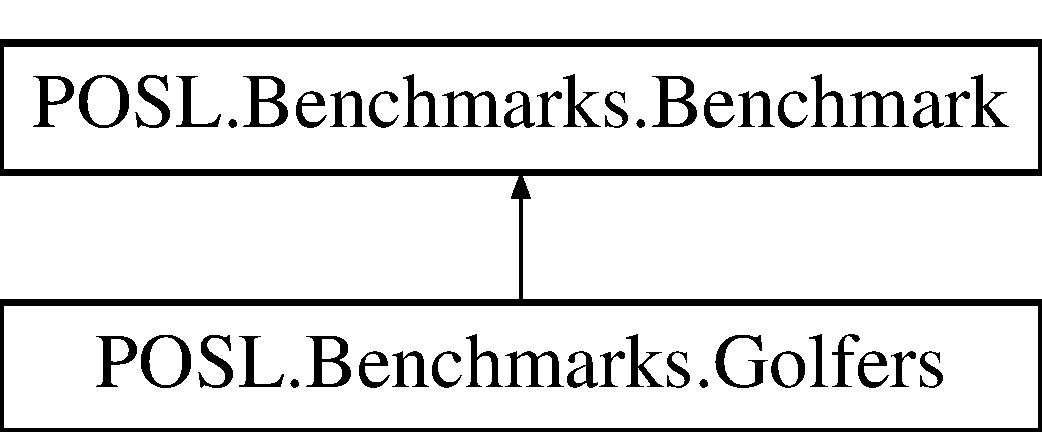
\includegraphics[height=2.000000cm]{classPOSL_1_1Benchmarks_1_1Benchmark}
\end{center}
\end{figure}
\subsection*{Public Member Functions}
\begin{DoxyCompactItemize}
\item 
\mbox{\Hypertarget{classPOSL_1_1Benchmarks_1_1Benchmark_ae548e466c0be888895a5009429932201}\label{classPOSL_1_1Benchmarks_1_1Benchmark_ae548e466c0be888895a5009429932201}} 
{\bfseries Benchmark} (int \+\_\+dimension, \hyperlink{classPOSL_1_1Domain}{Domain} \+\_\+domain, \hyperlink{interfacePOSL_1_1Benchmarks_1_1ICostStrategy}{I\+Cost\+Strategy} \+\_\+cost\+\_\+strategy, \hyperlink{interfacePOSL_1_1Benchmarks_1_1IRelativeCostStrategy}{I\+Relative\+Cost\+Strategy} \+\_\+relative\+\_\+cost\+\_\+strategy, \hyperlink{interfacePOSL_1_1Benchmarks_1_1IShowStrategy}{I\+Show\+Strategy} \+\_\+show\+\_\+strategy)
\item 
\mbox{\Hypertarget{classPOSL_1_1Benchmarks_1_1Benchmark_a3dfb4640f087374b57bd40337c8cc920}\label{classPOSL_1_1Benchmarks_1_1Benchmark_a3dfb4640f087374b57bd40337c8cc920}} 
int {\bfseries relative\+Solution\+Cost} (\hyperlink{classPOSL_1_1Data_1_1Solution}{Solution} solution)
\item 
\mbox{\Hypertarget{classPOSL_1_1Benchmarks_1_1Benchmark_ab488f070e3fec663718efaea87e92084}\label{classPOSL_1_1Benchmarks_1_1Benchmark_ab488f070e3fec663718efaea87e92084}} 
int {\bfseries relative\+Solution\+Cost} (\hyperlink{classPOSL_1_1Data_1_1Solution}{Solution} new\+\_\+solution, \hyperlink{structPOSL_1_1Tools_1_1T__Changes}{T\+\_\+\+Changes} changes)
\item 
\mbox{\Hypertarget{classPOSL_1_1Benchmarks_1_1Benchmark_a4be37728713fb268d139bc0a1b98a654}\label{classPOSL_1_1Benchmarks_1_1Benchmark_a4be37728713fb268d139bc0a1b98a654}} 
int {\bfseries solution\+Cost} (\hyperlink{classPOSL_1_1Data_1_1Solution}{Solution} solution)
\item 
\mbox{\Hypertarget{classPOSL_1_1Benchmarks_1_1Benchmark_a2000f8bd97b5e5c39a5a4dfd9796336c}\label{classPOSL_1_1Benchmarks_1_1Benchmark_a2000f8bd97b5e5c39a5a4dfd9796336c}} 
string {\bfseries Show\+Solution} (\hyperlink{classPOSL_1_1Data_1_1Solution}{Solution} solution)
\item 
\mbox{\Hypertarget{classPOSL_1_1Benchmarks_1_1Benchmark_a17f3f8597ab08be6a36bdc9216ec7cb4}\label{classPOSL_1_1Benchmarks_1_1Benchmark_a17f3f8597ab08be6a36bdc9216ec7cb4}} 
void {\bfseries Initialize\+Cost\+Data} (\hyperlink{classPOSL_1_1Data_1_1Solution}{Solution} solution)
\item 
\mbox{\Hypertarget{classPOSL_1_1Benchmarks_1_1Benchmark_aed1c0227427e7273345f1ee4d488187c}\label{classPOSL_1_1Benchmarks_1_1Benchmark_aed1c0227427e7273345f1ee4d488187c}} 
void {\bfseries Update\+Solution} (\hyperlink{classPOSL_1_1Data_1_1Solution}{Solution} solution)
\item 
\mbox{\Hypertarget{classPOSL_1_1Benchmarks_1_1Benchmark_aa38139d8ca8256f00f1e94630c71d1b1}\label{classPOSL_1_1Benchmarks_1_1Benchmark_aa38139d8ca8256f00f1e94630c71d1b1}} 
int {\bfseries cost\+On\+Variable} (int index)
\item 
\mbox{\Hypertarget{classPOSL_1_1Benchmarks_1_1Benchmark_a733060374289829c365ea2f8e8b2b7b9}\label{classPOSL_1_1Benchmarks_1_1Benchmark_a733060374289829c365ea2f8e8b2b7b9}} 
int {\bfseries sickest\+Variable} ()
\item 
\mbox{\Hypertarget{classPOSL_1_1Benchmarks_1_1Benchmark_aa47acbe1782a1ffa923c8c8b032010f9}\label{classPOSL_1_1Benchmarks_1_1Benchmark_aa47acbe1782a1ffa923c8c8b032010f9}} 
virtual int \mbox{[}$\,$\mbox{]} {\bfseries Reset} ()
\item 
\mbox{\Hypertarget{classPOSL_1_1Benchmarks_1_1Benchmark_a067bd6b6146982adc30a6962e4661660}\label{classPOSL_1_1Benchmarks_1_1Benchmark_a067bd6b6146982adc30a6962e4661660}} 
abstract string {\bfseries show\+Instance} ()
\end{DoxyCompactItemize}
\subsection*{Protected Attributes}
\begin{DoxyCompactItemize}
\item 
\mbox{\Hypertarget{classPOSL_1_1Benchmarks_1_1Benchmark_ae3e235947274b603a2211dc44c15ff83}\label{classPOSL_1_1Benchmarks_1_1Benchmark_ae3e235947274b603a2211dc44c15ff83}} 
int {\bfseries problem\+\_\+dimension}
\item 
\mbox{\Hypertarget{classPOSL_1_1Benchmarks_1_1Benchmark_a935568da14ba382b8287baac1eebbd72}\label{classPOSL_1_1Benchmarks_1_1Benchmark_a935568da14ba382b8287baac1eebbd72}} 
\hyperlink{classPOSL_1_1Domain}{Domain} {\bfseries domain}
\item 
\mbox{\Hypertarget{classPOSL_1_1Benchmarks_1_1Benchmark_ae9c7cd16c5befdf856a7dd7d4e7a824e}\label{classPOSL_1_1Benchmarks_1_1Benchmark_ae9c7cd16c5befdf856a7dd7d4e7a824e}} 
int \mbox{[}$\,$\mbox{]} {\bfseries configuration}
\item 
\mbox{\Hypertarget{classPOSL_1_1Benchmarks_1_1Benchmark_affe8324dcf208faa5a96d21ad452ecfb}\label{classPOSL_1_1Benchmarks_1_1Benchmark_affe8324dcf208faa5a96d21ad452ecfb}} 
int \mbox{[}$\,$\mbox{]} {\bfseries default\+\_\+configuration}
\item 
\mbox{\Hypertarget{classPOSL_1_1Benchmarks_1_1Benchmark_ad4d2d44386496a9df0ad20ade8f50ce7}\label{classPOSL_1_1Benchmarks_1_1Benchmark_ad4d2d44386496a9df0ad20ade8f50ce7}} 
\hyperlink{interfacePOSL_1_1Benchmarks_1_1ICostStrategy}{I\+Cost\+Strategy} \hyperlink{classPOSL_1_1Benchmarks_1_1Benchmark_ad4d2d44386496a9df0ad20ade8f50ce7}{cost\+\_\+strategy}
\begin{DoxyCompactList}\small\item\em S\+T\+R\+A\+T\+E\+G\+I\+ES. \end{DoxyCompactList}\item 
\mbox{\Hypertarget{classPOSL_1_1Benchmarks_1_1Benchmark_a1cf12bd559af07704a90e30e911f80a4}\label{classPOSL_1_1Benchmarks_1_1Benchmark_a1cf12bd559af07704a90e30e911f80a4}} 
\hyperlink{interfacePOSL_1_1Benchmarks_1_1IRelativeCostStrategy}{I\+Relative\+Cost\+Strategy} {\bfseries relative\+\_\+cost\+\_\+strategy}
\item 
\mbox{\Hypertarget{classPOSL_1_1Benchmarks_1_1Benchmark_a7ff725396b155958d8ec2359d565da26}\label{classPOSL_1_1Benchmarks_1_1Benchmark_a7ff725396b155958d8ec2359d565da26}} 
\hyperlink{interfacePOSL_1_1Benchmarks_1_1IShowStrategy}{I\+Show\+Strategy} {\bfseries show\+\_\+strategy}
\end{DoxyCompactItemize}
\subsection*{Properties}
\begin{DoxyCompactItemize}
\item 
\mbox{\Hypertarget{classPOSL_1_1Benchmarks_1_1Benchmark_a430d199f3d0bf357b43f876deb380110}\label{classPOSL_1_1Benchmarks_1_1Benchmark_a430d199f3d0bf357b43f876deb380110}} 
int {\bfseries Dimension}\hspace{0.3cm}{\ttfamily  \mbox{[}get\mbox{]}}
\item 
\mbox{\Hypertarget{classPOSL_1_1Benchmarks_1_1Benchmark_abe0aa39dceb516506b4f61f989bc78fe}\label{classPOSL_1_1Benchmarks_1_1Benchmark_abe0aa39dceb516506b4f61f989bc78fe}} 
\hyperlink{classPOSL_1_1Domain}{Domain} {\bfseries Variable\+\_\+\+Domain}\hspace{0.3cm}{\ttfamily  \mbox{[}get\mbox{]}}
\item 
\mbox{\Hypertarget{classPOSL_1_1Benchmarks_1_1Benchmark_a2fed212788c95bfe98d2a47b6a05cb82}\label{classPOSL_1_1Benchmarks_1_1Benchmark_a2fed212788c95bfe98d2a47b6a05cb82}} 
int {\bfseries Current\+Cost}\hspace{0.3cm}{\ttfamily  \mbox{[}get\mbox{]}}
\item 
\mbox{\Hypertarget{classPOSL_1_1Benchmarks_1_1Benchmark_a25c6ad71eaeee07eec0578d8ffff148e}\label{classPOSL_1_1Benchmarks_1_1Benchmark_a25c6ad71eaeee07eec0578d8ffff148e}} 
\hyperlink{classPOSL_1_1Data_1_1Solution}{Solution} {\bfseries Get\+Solution}\hspace{0.3cm}{\ttfamily  \mbox{[}get\mbox{]}}
\end{DoxyCompactItemize}


\subsection{Detailed Description}
(Abstract) Class to represent an instance of a problem 

The documentation for this class was generated from the following file\+:\begin{DoxyCompactItemize}
\item 
P\+O\+S\+L/\+P\+O\+S\+L/\+Benchmark/Benchmark.\+cs\end{DoxyCompactItemize}

\hypertarget{classPOSL_1_1Data_1_1ComputationData}{}\section{P\+O\+S\+L.\+Data.\+Computation\+Data Class Reference}
\label{classPOSL_1_1Data_1_1ComputationData}\index{P\+O\+S\+L.\+Data.\+Computation\+Data@{P\+O\+S\+L.\+Data.\+Computation\+Data}}


(Abstract) Class to represent all types of I/O in \hyperlink{namespacePOSL}{P\+O\+SL}  


Inheritance diagram for P\+O\+S\+L.\+Data.\+Computation\+Data\+:\begin{figure}[H]
\begin{center}
\leavevmode
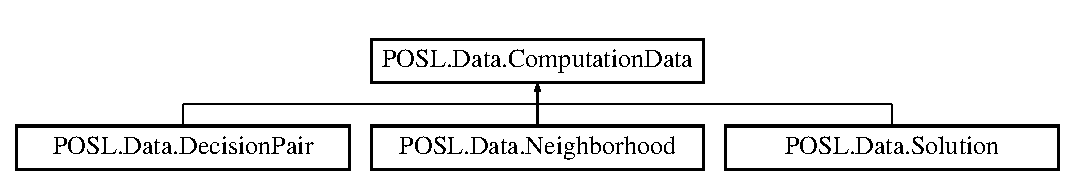
\includegraphics[height=2.000000cm]{classPOSL_1_1Data_1_1ComputationData}
\end{center}
\end{figure}
\subsection*{Public Member Functions}
\begin{DoxyCompactItemize}
\item 
\mbox{\Hypertarget{classPOSL_1_1Data_1_1ComputationData_ae347eba974b43e63f1aa984ef7475f9d}\label{classPOSL_1_1Data_1_1ComputationData_ae347eba974b43e63f1aa984ef7475f9d}} 
abstract string {\bfseries Tag} ()
\item 
abstract int \hyperlink{classPOSL_1_1Data_1_1ComputationData_a6cca889bb4ce32104d91dba413ef8c56}{comapare\+To} (\hyperlink{classPOSL_1_1Data_1_1ComputationData}{Computation\+Data} other, Func$<$ \hyperlink{classPOSL_1_1Data_1_1ComputationData}{Computation\+Data}, int $>$ criteria)
\begin{DoxyCompactList}\small\item\em Compare this object with other, given a function (criteria) \end{DoxyCompactList}\end{DoxyCompactItemize}


\subsection{Detailed Description}
(Abstract) Class to represent all types of I/O in \hyperlink{namespacePOSL}{P\+O\+SL} 

\subsection{Member Function Documentation}
\mbox{\Hypertarget{classPOSL_1_1Data_1_1ComputationData_a6cca889bb4ce32104d91dba413ef8c56}\label{classPOSL_1_1Data_1_1ComputationData_a6cca889bb4ce32104d91dba413ef8c56}} 
\index{P\+O\+S\+L\+::\+Data\+::\+Computation\+Data@{P\+O\+S\+L\+::\+Data\+::\+Computation\+Data}!comapare\+To@{comapare\+To}}
\index{comapare\+To@{comapare\+To}!P\+O\+S\+L\+::\+Data\+::\+Computation\+Data@{P\+O\+S\+L\+::\+Data\+::\+Computation\+Data}}
\subsubsection{\texorpdfstring{comapare\+To()}{comapareTo()}}
{\footnotesize\ttfamily abstract int P\+O\+S\+L.\+Data.\+Computation\+Data.\+comapare\+To (\begin{DoxyParamCaption}\item[{\hyperlink{classPOSL_1_1Data_1_1ComputationData}{Computation\+Data}}]{other,  }\item[{Func$<$ \hyperlink{classPOSL_1_1Data_1_1ComputationData}{Computation\+Data}, int $>$}]{criteria }\end{DoxyParamCaption})\hspace{0.3cm}{\ttfamily [pure virtual]}}



Compare this object with other, given a function (criteria) 


\begin{DoxyParams}{Parameters}
{\em other} & The \hyperlink{classPOSL_1_1Data_1_1ComputationData}{Computation\+Data} to compare with. \\
\hline
{\em criteria} & A function (criteria). \\
\hline
\end{DoxyParams}
\begin{DoxyReturn}{Returns}
-\/1 if T\+H\+IS is lower, 1 if T\+H\+IS is bigger, 0 if equals 
\end{DoxyReturn}


Implemented in \hyperlink{classPOSL_1_1Data_1_1Solution_a17d810433104964cc43bf65f35d25cc7}{P\+O\+S\+L.\+Data.\+Solution}, \hyperlink{classPOSL_1_1Data_1_1DecisionPair_a86eb9f86339a60733443d1fd1332913d}{P\+O\+S\+L.\+Data.\+Decision\+Pair}, and \hyperlink{classPOSL_1_1Data_1_1Neighborhood_aa7014a3cbaf532f49d89468c20b7c269}{P\+O\+S\+L.\+Data.\+Neighborhood}.



The documentation for this class was generated from the following file\+:\begin{DoxyCompactItemize}
\item 
P\+O\+S\+L/\+P\+O\+S\+L/\+Data/Computation\+Data.\+cs\end{DoxyCompactItemize}

\hypertarget{classPOSL_1_1Tools_1_1ConnectionMatrix}{}\section{P\+O\+S\+L.\+Tools.\+Connection\+Matrix Class Reference}
\label{classPOSL_1_1Tools_1_1ConnectionMatrix}\index{P\+O\+S\+L.\+Tools.\+Connection\+Matrix@{P\+O\+S\+L.\+Tools.\+Connection\+Matrix}}
\subsection*{Public Member Functions}
\begin{DoxyCompactItemize}
\item 
\mbox{\Hypertarget{classPOSL_1_1Tools_1_1ConnectionMatrix_a0eca15eb6b4a326ba28fca14ef23d9cd}\label{classPOSL_1_1Tools_1_1ConnectionMatrix_a0eca15eb6b4a326ba28fca14ef23d9cd}} 
{\bfseries Connection\+Matrix} (int n)
\item 
\mbox{\Hypertarget{classPOSL_1_1Tools_1_1ConnectionMatrix_a70b7d98c6c3adc0a9ef316109e0e3694}\label{classPOSL_1_1Tools_1_1ConnectionMatrix_a70b7d98c6c3adc0a9ef316109e0e3694}} 
int {\bfseries add\+\_\+connection} (int a, int b, bool updating)
\item 
\mbox{\Hypertarget{classPOSL_1_1Tools_1_1ConnectionMatrix_a3538acc9b3491f308c68a8eb92e23152}\label{classPOSL_1_1Tools_1_1ConnectionMatrix_a3538acc9b3491f308c68a8eb92e23152}} 
int {\bfseries remove\+\_\+connection} (int a, int b, bool updating)
\item 
\mbox{\Hypertarget{classPOSL_1_1Tools_1_1ConnectionMatrix_a224493020bd1c4e5b6281ded7f3222c5}\label{classPOSL_1_1Tools_1_1ConnectionMatrix_a224493020bd1c4e5b6281ded7f3222c5}} 
int {\bfseries get\+\_\+connectios} (int a, int b)
\item 
\mbox{\Hypertarget{classPOSL_1_1Tools_1_1ConnectionMatrix_ac6063f7933c40c5b33b35ffb6b14816b}\label{classPOSL_1_1Tools_1_1ConnectionMatrix_ac6063f7933c40c5b33b35ffb6b14816b}} 
int {\bfseries ranking\+\_\+cost\+\_\+of\+\_\+variable} (int variable\+\_\+index)
\item 
\mbox{\Hypertarget{classPOSL_1_1Tools_1_1ConnectionMatrix_a85cd79597c9d79e11f27524a7aebdc79}\label{classPOSL_1_1Tools_1_1ConnectionMatrix_a85cd79597c9d79e11f27524a7aebdc79}} 
int {\bfseries projected\+\_\+cost} (int a, int b)
\item 
\mbox{\Hypertarget{classPOSL_1_1Tools_1_1ConnectionMatrix_a45aa862703300f0837bdb535282ff237}\label{classPOSL_1_1Tools_1_1ConnectionMatrix_a45aa862703300f0837bdb535282ff237}} 
void {\bfseries clear} ()
\end{DoxyCompactItemize}


The documentation for this class was generated from the following file\+:\begin{DoxyCompactItemize}
\item 
P\+O\+S\+L/\+P\+O\+S\+L/\+Tools/Connection\+Matrix.\+cs\end{DoxyCompactItemize}

\hypertarget{classPOSL_1_1Data_1_1DecisionPair}{}\section{P\+O\+S\+L.\+Data.\+Decision\+Pair Class Reference}
\label{classPOSL_1_1Data_1_1DecisionPair}\index{P\+O\+S\+L.\+Data.\+Decision\+Pair@{P\+O\+S\+L.\+Data.\+Decision\+Pair}}


Class to represent a couple of solutions (current and new found)  


Inheritance diagram for P\+O\+S\+L.\+Data.\+Decision\+Pair\+:\begin{figure}[H]
\begin{center}
\leavevmode
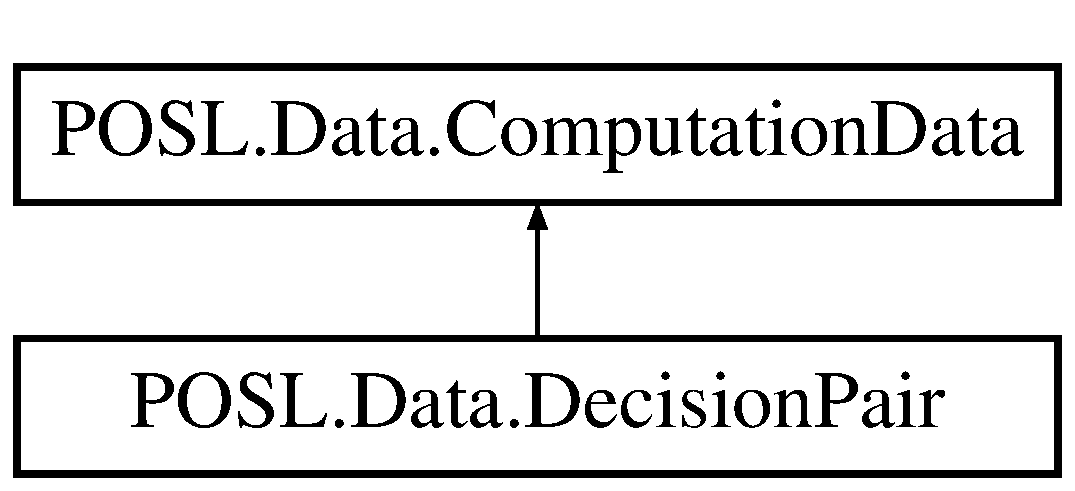
\includegraphics[height=2.000000cm]{classPOSL_1_1Data_1_1DecisionPair}
\end{center}
\end{figure}
\subsection*{Public Member Functions}
\begin{DoxyCompactItemize}
\item 
\mbox{\Hypertarget{classPOSL_1_1Data_1_1DecisionPair_a4f788fe41311016d6dddf877d9d6242a}\label{classPOSL_1_1Data_1_1DecisionPair_a4f788fe41311016d6dddf877d9d6242a}} 
override string {\bfseries Tag} ()
\item 
\mbox{\Hypertarget{classPOSL_1_1Data_1_1DecisionPair_ae46b40ebacd27dabc909d32c7bd607e0}\label{classPOSL_1_1Data_1_1DecisionPair_ae46b40ebacd27dabc909d32c7bd607e0}} 
{\bfseries Decision\+Pair} (\hyperlink{classPOSL_1_1Data_1_1Solution}{Solution} \+\_\+current, \hyperlink{classPOSL_1_1Data_1_1Solution}{Solution} \+\_\+found)
\item 
\mbox{\Hypertarget{classPOSL_1_1Data_1_1DecisionPair_a60666eb915fc24969228af5603eb0447}\label{classPOSL_1_1Data_1_1DecisionPair_a60666eb915fc24969228af5603eb0447}} 
bool {\bfseries Both\+Equals} ()
\item 
\mbox{\Hypertarget{classPOSL_1_1Data_1_1DecisionPair_a28598b5e6693c16d43417d445a3ba47b}\label{classPOSL_1_1Data_1_1DecisionPair_a28598b5e6693c16d43417d445a3ba47b}} 
override bool {\bfseries Equals} (object other)
\item 
\mbox{\Hypertarget{classPOSL_1_1Data_1_1DecisionPair_adb91932988131b145473d3d3391c4a59}\label{classPOSL_1_1Data_1_1DecisionPair_adb91932988131b145473d3d3391c4a59}} 
override int {\bfseries Get\+Hash\+Code} ()
\item 
override int \hyperlink{classPOSL_1_1Data_1_1DecisionPair_a86eb9f86339a60733443d1fd1332913d}{comapare\+To} (\hyperlink{classPOSL_1_1Data_1_1ComputationData}{Computation\+Data} other, Func$<$ \hyperlink{classPOSL_1_1Data_1_1ComputationData}{Computation\+Data}, int $>$ criteria)
\begin{DoxyCompactList}\small\item\em Compare this object with other, given a function (criteria) \end{DoxyCompactList}\end{DoxyCompactItemize}
\subsection*{Properties}
\begin{DoxyCompactItemize}
\item 
\mbox{\Hypertarget{classPOSL_1_1Data_1_1DecisionPair_a7757ed873d87b365b39f7ec3b203b428}\label{classPOSL_1_1Data_1_1DecisionPair_a7757ed873d87b365b39f7ec3b203b428}} 
\hyperlink{classPOSL_1_1Data_1_1Solution}{Solution} {\bfseries Get\+Current}\hspace{0.3cm}{\ttfamily  \mbox{[}get\mbox{]}}
\item 
\mbox{\Hypertarget{classPOSL_1_1Data_1_1DecisionPair_a57e8d7fbe6e4e9ef9371aefd5e061627}\label{classPOSL_1_1Data_1_1DecisionPair_a57e8d7fbe6e4e9ef9371aefd5e061627}} 
\hyperlink{classPOSL_1_1Data_1_1Solution}{Solution} {\bfseries Get\+Found}\hspace{0.3cm}{\ttfamily  \mbox{[}get\mbox{]}}
\item 
\mbox{\Hypertarget{classPOSL_1_1Data_1_1DecisionPair_ae5b43d45b945d7c4a5f3fb6433ade45e}\label{classPOSL_1_1Data_1_1DecisionPair_ae5b43d45b945d7c4a5f3fb6433ade45e}} 
string {\bfseries Solution\+Packing\+ID}\hspace{0.3cm}{\ttfamily  \mbox{[}get\mbox{]}}
\end{DoxyCompactItemize}


\subsection{Detailed Description}
Class to represent a couple of solutions (current and new found) 

\subsection{Member Function Documentation}
\mbox{\Hypertarget{classPOSL_1_1Data_1_1DecisionPair_a86eb9f86339a60733443d1fd1332913d}\label{classPOSL_1_1Data_1_1DecisionPair_a86eb9f86339a60733443d1fd1332913d}} 
\index{P\+O\+S\+L\+::\+Data\+::\+Decision\+Pair@{P\+O\+S\+L\+::\+Data\+::\+Decision\+Pair}!comapare\+To@{comapare\+To}}
\index{comapare\+To@{comapare\+To}!P\+O\+S\+L\+::\+Data\+::\+Decision\+Pair@{P\+O\+S\+L\+::\+Data\+::\+Decision\+Pair}}
\subsubsection{\texorpdfstring{comapare\+To()}{comapareTo()}}
{\footnotesize\ttfamily override int P\+O\+S\+L.\+Data.\+Decision\+Pair.\+comapare\+To (\begin{DoxyParamCaption}\item[{\hyperlink{classPOSL_1_1Data_1_1ComputationData}{Computation\+Data}}]{other,  }\item[{Func$<$ \hyperlink{classPOSL_1_1Data_1_1ComputationData}{Computation\+Data}, int $>$}]{criteria }\end{DoxyParamCaption})\hspace{0.3cm}{\ttfamily [inline]}, {\ttfamily [virtual]}}



Compare this object with other, given a function (criteria) 


\begin{DoxyParams}{Parameters}
{\em other} & The \hyperlink{classPOSL_1_1Data_1_1ComputationData}{Computation\+Data} to compare with. \\
\hline
{\em criteria} & A function (criteria). \\
\hline
\end{DoxyParams}
\begin{DoxyReturn}{Returns}
-\/1 if T\+H\+IS is lower, 1 if T\+H\+IS is bigger, 0 if equals 
\end{DoxyReturn}


Implements \hyperlink{classPOSL_1_1Data_1_1ComputationData_a6cca889bb4ce32104d91dba413ef8c56}{P\+O\+S\+L.\+Data.\+Computation\+Data}.



The documentation for this class was generated from the following file\+:\begin{DoxyCompactItemize}
\item 
P\+O\+S\+L/\+P\+O\+S\+L/\+Data/Decision\+Pair.\+cs\end{DoxyCompactItemize}

\hypertarget{classPOSL_1_1Domain}{}\section{P\+O\+S\+L.\+Domain Class Reference}
\label{classPOSL_1_1Domain}\index{P\+O\+S\+L.\+Domain@{P\+O\+S\+L.\+Domain}}
Inheritance diagram for P\+O\+S\+L.\+Domain\+:\begin{figure}[H]
\begin{center}
\leavevmode
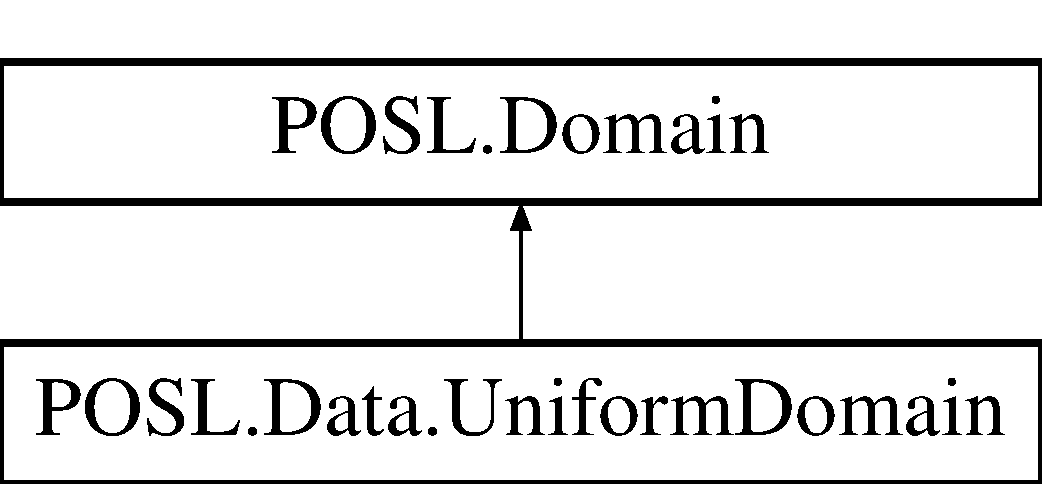
\includegraphics[height=2.000000cm]{classPOSL_1_1Domain}
\end{center}
\end{figure}
\subsection*{Public Member Functions}
\begin{DoxyCompactItemize}
\item 
\mbox{\Hypertarget{classPOSL_1_1Domain_a922d6ee4f986156f642a6e2329fd2342}\label{classPOSL_1_1Domain_a922d6ee4f986156f642a6e2329fd2342}} 
abstract int \mbox{[}$\,$\mbox{]} {\bfseries Get\+Values} (int variable)
\item 
\mbox{\Hypertarget{classPOSL_1_1Domain_ac4499b68d14f91a16e9a6c3a59daed4f}\label{classPOSL_1_1Domain_ac4499b68d14f91a16e9a6c3a59daed4f}} 
abstract int {\bfseries minimum} (int variable)
\item 
\mbox{\Hypertarget{classPOSL_1_1Domain_a2bfcaefd8f65cb4212d6457cefec7d2b}\label{classPOSL_1_1Domain_a2bfcaefd8f65cb4212d6457cefec7d2b}} 
abstract int {\bfseries maximum} (int variable)
\end{DoxyCompactItemize}


The documentation for this class was generated from the following file\+:\begin{DoxyCompactItemize}
\item 
P\+O\+S\+L/\+P\+O\+S\+L/\+Data/Domain.\+cs\end{DoxyCompactItemize}

\hypertarget{classPOSL_1_1Data_1_1ElementsChangeIterator}{}\section{P\+O\+S\+L.\+Data.\+Elements\+Change\+Iterator Class Reference}
\label{classPOSL_1_1Data_1_1ElementsChangeIterator}\index{P\+O\+S\+L.\+Data.\+Elements\+Change\+Iterator@{P\+O\+S\+L.\+Data.\+Elements\+Change\+Iterator}}
Inheritance diagram for P\+O\+S\+L.\+Data.\+Elements\+Change\+Iterator\+:\begin{figure}[H]
\begin{center}
\leavevmode
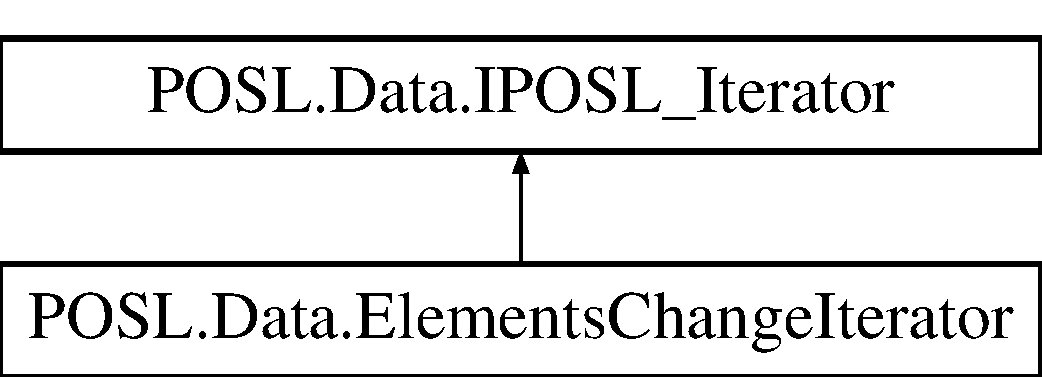
\includegraphics[height=2.000000cm]{classPOSL_1_1Data_1_1ElementsChangeIterator}
\end{center}
\end{figure}
\subsection*{Public Member Functions}
\begin{DoxyCompactItemize}
\item 
\mbox{\Hypertarget{classPOSL_1_1Data_1_1ElementsChangeIterator_aeaea7a035bb28c9d052d6eb9fe976d57}\label{classPOSL_1_1Data_1_1ElementsChangeIterator_aeaea7a035bb28c9d052d6eb9fe976d57}} 
{\bfseries Elements\+Change\+Iterator} (\hyperlink{classPOSL_1_1Data_1_1Neighborhood}{Neighborhood} \+\_\+n)
\item 
\mbox{\Hypertarget{classPOSL_1_1Data_1_1ElementsChangeIterator_a506e0b82b8c3072082536d2aa3ff8c90}\label{classPOSL_1_1Data_1_1ElementsChangeIterator_a506e0b82b8c3072082536d2aa3ff8c90}} 
int \mbox{[}$\,$\mbox{]} {\bfseries Get\+Next} ()
\item 
\mbox{\Hypertarget{classPOSL_1_1Data_1_1ElementsChangeIterator_aa8c7f76b149ed5bb6a6853bfbab1700f}\label{classPOSL_1_1Data_1_1ElementsChangeIterator_aa8c7f76b149ed5bb6a6853bfbab1700f}} 
bool {\bfseries Some\+Next} ()
\item 
\mbox{\Hypertarget{classPOSL_1_1Data_1_1ElementsChangeIterator_af8e33b308ccd1529bc244979c097e58d}\label{classPOSL_1_1Data_1_1ElementsChangeIterator_af8e33b308ccd1529bc244979c097e58d}} 
void {\bfseries Reset} ()
\end{DoxyCompactItemize}


The documentation for this class was generated from the following file\+:\begin{DoxyCompactItemize}
\item 
P\+O\+S\+L/\+P\+O\+S\+L/\+Data/data\+\_\+strategy/Elements\+Change\+Iterator.\+cs\end{DoxyCompactItemize}

\hypertarget{classPOSL_1_1Benchmarks_1_1Golfers}{}\section{P\+O\+S\+L.\+Benchmarks.\+Golfers Class Reference}
\label{classPOSL_1_1Benchmarks_1_1Golfers}\index{P\+O\+S\+L.\+Benchmarks.\+Golfers@{P\+O\+S\+L.\+Benchmarks.\+Golfers}}


Class to represent an instance of a \hyperlink{classPOSL_1_1Benchmarks_1_1Golfers}{Golfers} Problems.  


Inheritance diagram for P\+O\+S\+L.\+Benchmarks.\+Golfers\+:\begin{figure}[H]
\begin{center}
\leavevmode
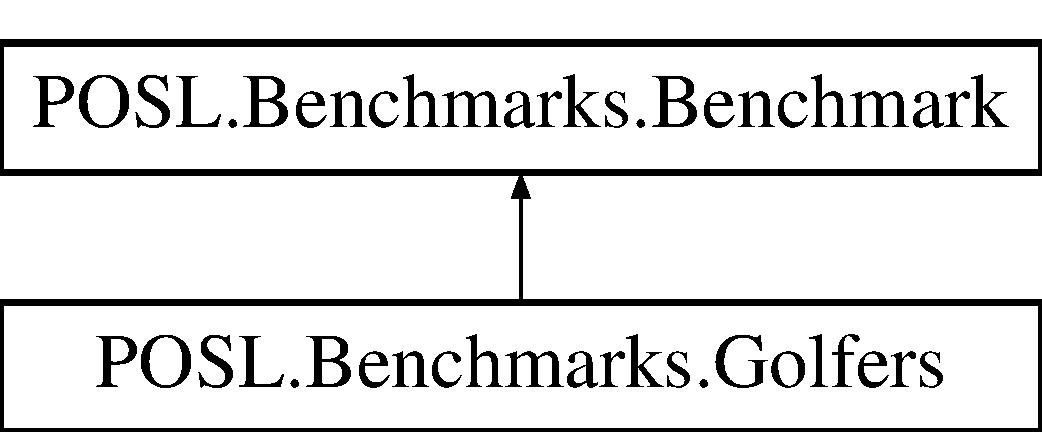
\includegraphics[height=2.000000cm]{classPOSL_1_1Benchmarks_1_1Golfers}
\end{center}
\end{figure}
\subsection*{Public Member Functions}
\begin{DoxyCompactItemize}
\item 
\mbox{\Hypertarget{classPOSL_1_1Benchmarks_1_1Golfers_ad094261c60bf502f8324d4bca0086271}\label{classPOSL_1_1Benchmarks_1_1Golfers_ad094261c60bf502f8324d4bca0086271}} 
{\bfseries Golfers} (int g, int p, int w)
\item 
\mbox{\Hypertarget{classPOSL_1_1Benchmarks_1_1Golfers_a657477c47bc09d1cb33780670a83d70d}\label{classPOSL_1_1Benchmarks_1_1Golfers_a657477c47bc09d1cb33780670a83d70d}} 
override string {\bfseries show\+Instance} ()
\end{DoxyCompactItemize}
\subsection*{Additional Inherited Members}


\subsection{Detailed Description}
Class to represent an instance of a \hyperlink{classPOSL_1_1Benchmarks_1_1Golfers}{Golfers} Problems. 

The documentation for this class was generated from the following file\+:\begin{DoxyCompactItemize}
\item 
P\+O\+S\+L/\+P\+O\+S\+L/\+Benchmark/Golfers.\+cs\end{DoxyCompactItemize}

\hypertarget{classPOSL_1_1Benchmarks_1_1GolfersDefaultShowStrategy}{}\section{P\+O\+S\+L.\+Benchmarks.\+Golfers\+Default\+Show\+Strategy Class Reference}
\label{classPOSL_1_1Benchmarks_1_1GolfersDefaultShowStrategy}\index{P\+O\+S\+L.\+Benchmarks.\+Golfers\+Default\+Show\+Strategy@{P\+O\+S\+L.\+Benchmarks.\+Golfers\+Default\+Show\+Strategy}}


Class to represent the way Social \hyperlink{classPOSL_1_1Benchmarks_1_1Golfers}{Golfers} problem shows its result (solution)  


Inheritance diagram for P\+O\+S\+L.\+Benchmarks.\+Golfers\+Default\+Show\+Strategy\+:\begin{figure}[H]
\begin{center}
\leavevmode
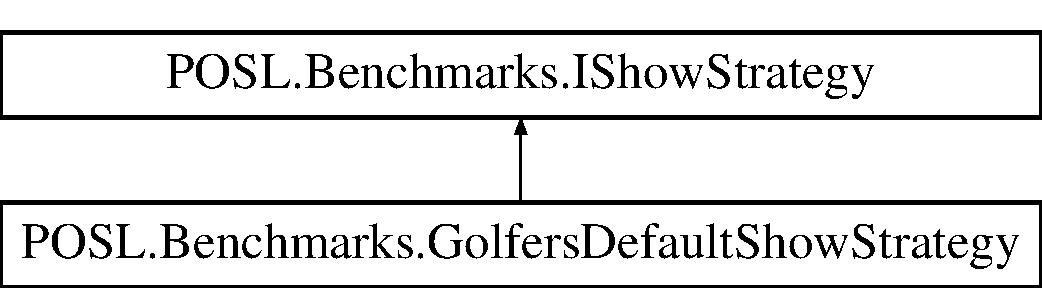
\includegraphics[height=2.000000cm]{classPOSL_1_1Benchmarks_1_1GolfersDefaultShowStrategy}
\end{center}
\end{figure}
\subsection*{Public Member Functions}
\begin{DoxyCompactItemize}
\item 
\hyperlink{classPOSL_1_1Benchmarks_1_1GolfersDefaultShowStrategy_aabef047e1ad34907123912f9cebb35fd}{Golfers\+Default\+Show\+Strategy} (int \+\_\+groups, int \+\_\+players, int \+\_\+weeks)
\begin{DoxyCompactList}\small\item\em Default constructor. \end{DoxyCompactList}\item 
\mbox{\Hypertarget{classPOSL_1_1Benchmarks_1_1GolfersDefaultShowStrategy_af4af1bde7fadcbf8e75a6b679676b0c8}\label{classPOSL_1_1Benchmarks_1_1GolfersDefaultShowStrategy_af4af1bde7fadcbf8e75a6b679676b0c8}} 
string \hyperlink{classPOSL_1_1Benchmarks_1_1GolfersDefaultShowStrategy_af4af1bde7fadcbf8e75a6b679676b0c8}{show\+Solution} (\hyperlink{classPOSL_1_1Data_1_1Solution}{Solution} solution)
\begin{DoxyCompactList}\small\item\em From $<$\+I\+Show\+Strategy$>$ \end{DoxyCompactList}\end{DoxyCompactItemize}


\subsection{Detailed Description}
Class to represent the way Social \hyperlink{classPOSL_1_1Benchmarks_1_1Golfers}{Golfers} problem shows its result (solution) 

\subsection{Constructor \& Destructor Documentation}
\mbox{\Hypertarget{classPOSL_1_1Benchmarks_1_1GolfersDefaultShowStrategy_aabef047e1ad34907123912f9cebb35fd}\label{classPOSL_1_1Benchmarks_1_1GolfersDefaultShowStrategy_aabef047e1ad34907123912f9cebb35fd}} 
\index{P\+O\+S\+L\+::\+Benchmarks\+::\+Golfers\+Default\+Show\+Strategy@{P\+O\+S\+L\+::\+Benchmarks\+::\+Golfers\+Default\+Show\+Strategy}!Golfers\+Default\+Show\+Strategy@{Golfers\+Default\+Show\+Strategy}}
\index{Golfers\+Default\+Show\+Strategy@{Golfers\+Default\+Show\+Strategy}!P\+O\+S\+L\+::\+Benchmarks\+::\+Golfers\+Default\+Show\+Strategy@{P\+O\+S\+L\+::\+Benchmarks\+::\+Golfers\+Default\+Show\+Strategy}}
\subsubsection{\texorpdfstring{Golfers\+Default\+Show\+Strategy()}{GolfersDefaultShowStrategy()}}
{\footnotesize\ttfamily P\+O\+S\+L.\+Benchmarks.\+Golfers\+Default\+Show\+Strategy.\+Golfers\+Default\+Show\+Strategy (\begin{DoxyParamCaption}\item[{int}]{\+\_\+groups,  }\item[{int}]{\+\_\+players,  }\item[{int}]{\+\_\+weeks }\end{DoxyParamCaption})\hspace{0.3cm}{\ttfamily [inline]}}



Default constructor. 


\begin{DoxyParams}{Parameters}
{\em \+\_\+groups} & Number of groups. \\
\hline
{\em \+\_\+players} & Number of players per gruop (total of players = \+\_\+groups $\ast$ \+\_\+players). \\
\hline
{\em \+\_\+weeks} & Number of weeks. \\
\hline
\end{DoxyParams}


The documentation for this class was generated from the following file\+:\begin{DoxyCompactItemize}
\item 
P\+O\+S\+L/\+P\+O\+S\+L/\+Benchmark/showing\+\_\+strategy/Golfers\+Default\+Show\+Strategy.\+cs\end{DoxyCompactItemize}

\hypertarget{classPOSL_1_1Benchmarks_1_1GolfersLongIntCostStrategy}{}\section{P\+O\+S\+L.\+Benchmarks.\+Golfers\+Long\+Int\+Cost\+Strategy Class Reference}
\label{classPOSL_1_1Benchmarks_1_1GolfersLongIntCostStrategy}\index{P\+O\+S\+L.\+Benchmarks.\+Golfers\+Long\+Int\+Cost\+Strategy@{P\+O\+S\+L.\+Benchmarks.\+Golfers\+Long\+Int\+Cost\+Strategy}}


Class to represent the absolute cost stratategy of Social Golgers Problem.  


Inheritance diagram for P\+O\+S\+L.\+Benchmarks.\+Golfers\+Long\+Int\+Cost\+Strategy\+:\begin{figure}[H]
\begin{center}
\leavevmode
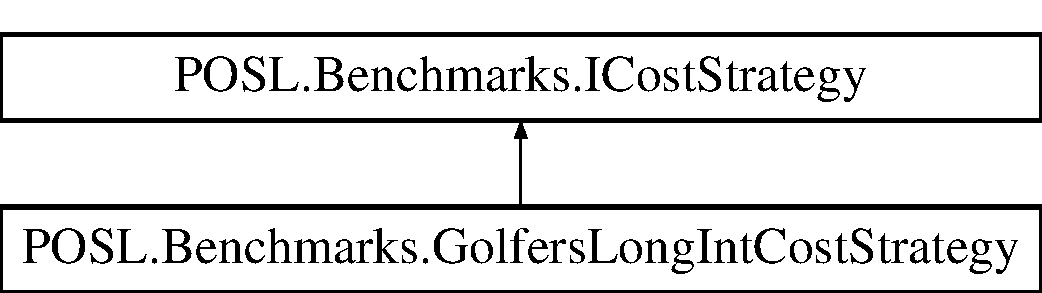
\includegraphics[height=2.000000cm]{classPOSL_1_1Benchmarks_1_1GolfersLongIntCostStrategy}
\end{center}
\end{figure}
\subsection*{Public Member Functions}
\begin{DoxyCompactItemize}
\item 
\hyperlink{classPOSL_1_1Benchmarks_1_1GolfersLongIntCostStrategy_af920964103d2261bcd0da265c7f06a55}{Golfers\+Long\+Int\+Cost\+Strategy} (int \+\_\+groups, int \+\_\+players, int \+\_\+weeks)
\begin{DoxyCompactList}\small\item\em Default constructor. \end{DoxyCompactList}\item 
\mbox{\Hypertarget{classPOSL_1_1Benchmarks_1_1GolfersLongIntCostStrategy_a44bd356a05ef5afcd158ba0e7b97a256}\label{classPOSL_1_1Benchmarks_1_1GolfersLongIntCostStrategy_a44bd356a05ef5afcd158ba0e7b97a256}} 
int {\bfseries solution\+Cost} (\hyperlink{classPOSL_1_1Data_1_1Solution}{Solution} solution)
\end{DoxyCompactItemize}


\subsection{Detailed Description}
Class to represent the absolute cost stratategy of Social Golgers Problem. 

\subsection{Constructor \& Destructor Documentation}
\mbox{\Hypertarget{classPOSL_1_1Benchmarks_1_1GolfersLongIntCostStrategy_af920964103d2261bcd0da265c7f06a55}\label{classPOSL_1_1Benchmarks_1_1GolfersLongIntCostStrategy_af920964103d2261bcd0da265c7f06a55}} 
\index{P\+O\+S\+L\+::\+Benchmarks\+::\+Golfers\+Long\+Int\+Cost\+Strategy@{P\+O\+S\+L\+::\+Benchmarks\+::\+Golfers\+Long\+Int\+Cost\+Strategy}!Golfers\+Long\+Int\+Cost\+Strategy@{Golfers\+Long\+Int\+Cost\+Strategy}}
\index{Golfers\+Long\+Int\+Cost\+Strategy@{Golfers\+Long\+Int\+Cost\+Strategy}!P\+O\+S\+L\+::\+Benchmarks\+::\+Golfers\+Long\+Int\+Cost\+Strategy@{P\+O\+S\+L\+::\+Benchmarks\+::\+Golfers\+Long\+Int\+Cost\+Strategy}}
\subsubsection{\texorpdfstring{Golfers\+Long\+Int\+Cost\+Strategy()}{GolfersLongIntCostStrategy()}}
{\footnotesize\ttfamily P\+O\+S\+L.\+Benchmarks.\+Golfers\+Long\+Int\+Cost\+Strategy.\+Golfers\+Long\+Int\+Cost\+Strategy (\begin{DoxyParamCaption}\item[{int}]{\+\_\+groups,  }\item[{int}]{\+\_\+players,  }\item[{int}]{\+\_\+weeks }\end{DoxyParamCaption})\hspace{0.3cm}{\ttfamily [inline]}}



Default constructor. 


\begin{DoxyParams}{Parameters}
{\em \+\_\+groups} & Number of groups. \\
\hline
{\em \+\_\+players} & Number of players per gruop (total of players = \+\_\+groups $\ast$ \+\_\+players). \\
\hline
{\em \+\_\+weeks} & Number of weeks. \\
\hline
\end{DoxyParams}


The documentation for this class was generated from the following file\+:\begin{DoxyCompactItemize}
\item 
P\+O\+S\+L/\+P\+O\+S\+L/\+Benchmark/cost\+\_\+strategy/Golfers\+Long\+Int\+Cost\+Strategy.\+cs\end{DoxyCompactItemize}

\hypertarget{classPOSL_1_1Benchmarks_1_1GolfersRelativeCostStrategy}{}\section{P\+O\+S\+L.\+Benchmarks.\+Golfers\+Relative\+Cost\+Strategy Class Reference}
\label{classPOSL_1_1Benchmarks_1_1GolfersRelativeCostStrategy}\index{P\+O\+S\+L.\+Benchmarks.\+Golfers\+Relative\+Cost\+Strategy@{P\+O\+S\+L.\+Benchmarks.\+Golfers\+Relative\+Cost\+Strategy}}
Inheritance diagram for P\+O\+S\+L.\+Benchmarks.\+Golfers\+Relative\+Cost\+Strategy\+:\begin{figure}[H]
\begin{center}
\leavevmode
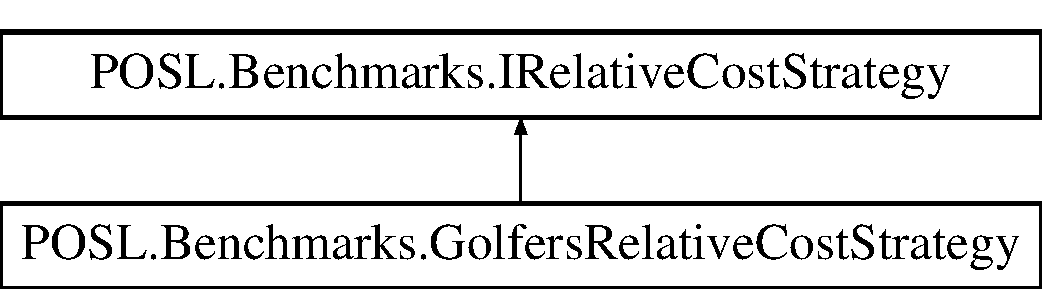
\includegraphics[height=2.000000cm]{classPOSL_1_1Benchmarks_1_1GolfersRelativeCostStrategy}
\end{center}
\end{figure}
\subsection*{Public Member Functions}
\begin{DoxyCompactItemize}
\item 
\mbox{\Hypertarget{classPOSL_1_1Benchmarks_1_1GolfersRelativeCostStrategy_a04e66ae4875f31dd4cf3cc7bb9c6628e}\label{classPOSL_1_1Benchmarks_1_1GolfersRelativeCostStrategy_a04e66ae4875f31dd4cf3cc7bb9c6628e}} 
{\bfseries Golfers\+Relative\+Cost\+Strategy} (int g, int p, int w)
\item 
\mbox{\Hypertarget{classPOSL_1_1Benchmarks_1_1GolfersRelativeCostStrategy_a8ca6815af453ac3bdac994568b1271aa}\label{classPOSL_1_1Benchmarks_1_1GolfersRelativeCostStrategy_a8ca6815af453ac3bdac994568b1271aa}} 
int \hyperlink{classPOSL_1_1Benchmarks_1_1GolfersRelativeCostStrategy_a8ca6815af453ac3bdac994568b1271aa}{current\+Cost} ()
\begin{DoxyCompactList}\small\item\em (Property) From $<$\+Relative\+Cost\+Strategy$>$ \end{DoxyCompactList}\item 
\mbox{\Hypertarget{classPOSL_1_1Benchmarks_1_1GolfersRelativeCostStrategy_a4cd8227c9b4cc4f3cc60025c0edc7f9f}\label{classPOSL_1_1Benchmarks_1_1GolfersRelativeCostStrategy_a4cd8227c9b4cc4f3cc60025c0edc7f9f}} 
void {\bfseries initialize\+Cost\+Data} (\hyperlink{classPOSL_1_1Data_1_1Solution}{Solution} solution, int \+\_\+initial\+\_\+cost)
\item 
\mbox{\Hypertarget{classPOSL_1_1Benchmarks_1_1GolfersRelativeCostStrategy_a11c9ae1e6798fd68965e2dfdc577e76b}\label{classPOSL_1_1Benchmarks_1_1GolfersRelativeCostStrategy_a11c9ae1e6798fd68965e2dfdc577e76b}} 
int {\bfseries relative\+\_\+cost} (\hyperlink{classPOSL_1_1Data_1_1Solution}{Solution} new\+\_\+solution, \hyperlink{structPOSL_1_1Tools_1_1T__Changes}{T\+\_\+\+Changes} change, bool updating)
\item 
\mbox{\Hypertarget{classPOSL_1_1Benchmarks_1_1GolfersRelativeCostStrategy_ab194469d5bd6f4a8139ae5794690515a}\label{classPOSL_1_1Benchmarks_1_1GolfersRelativeCostStrategy_ab194469d5bd6f4a8139ae5794690515a}} 
void {\bfseries update\+Configuration} (\hyperlink{classPOSL_1_1Data_1_1Solution}{Solution} new\+\_\+solution)
\item 
\mbox{\Hypertarget{classPOSL_1_1Benchmarks_1_1GolfersRelativeCostStrategy_afdb9cae8e34b3e99fab4ec3b7e01e7df}\label{classPOSL_1_1Benchmarks_1_1GolfersRelativeCostStrategy_afdb9cae8e34b3e99fab4ec3b7e01e7df}} 
int {\bfseries relative\+Solution\+Cost} (\hyperlink{classPOSL_1_1Data_1_1Solution}{Solution} new\+\_\+solution)
\item 
\mbox{\Hypertarget{classPOSL_1_1Benchmarks_1_1GolfersRelativeCostStrategy_a7955b5a608662c7a39684896f8475e8f}\label{classPOSL_1_1Benchmarks_1_1GolfersRelativeCostStrategy_a7955b5a608662c7a39684896f8475e8f}} 
int {\bfseries relative\+Solution\+Cost} (\hyperlink{classPOSL_1_1Data_1_1Solution}{Solution} new\+\_\+solution, \hyperlink{structPOSL_1_1Tools_1_1T__Changes}{T\+\_\+\+Changes} \+\_\+changes)
\item 
\mbox{\Hypertarget{classPOSL_1_1Benchmarks_1_1GolfersRelativeCostStrategy_a168f0a51067b3953c29d02b15f1b481d}\label{classPOSL_1_1Benchmarks_1_1GolfersRelativeCostStrategy_a168f0a51067b3953c29d02b15f1b481d}} 
int {\bfseries cost\+On\+Variable} (int variable\+\_\+index)
\item 
\mbox{\Hypertarget{classPOSL_1_1Benchmarks_1_1GolfersRelativeCostStrategy_a7662cbfa217153ef577767bbea22b559}\label{classPOSL_1_1Benchmarks_1_1GolfersRelativeCostStrategy_a7662cbfa217153ef577767bbea22b559}} 
int \hyperlink{classPOSL_1_1Benchmarks_1_1GolfersRelativeCostStrategy_a7662cbfa217153ef577767bbea22b559}{sickest\+Variable} ()
\begin{DoxyCompactList}\small\item\em Returns just the worst player. \end{DoxyCompactList}\end{DoxyCompactItemize}


The documentation for this class was generated from the following file\+:\begin{DoxyCompactItemize}
\item 
P\+O\+S\+L/\+P\+O\+S\+L/\+Benchmark/cost\+\_\+strategy/Golfers\+Relative\+Cost\+Strategy.\+cs\end{DoxyCompactItemize}

\hypertarget{interfacePOSL_1_1Benchmarks_1_1ICostStrategy}{}\section{P\+O\+S\+L.\+Benchmarks.\+I\+Cost\+Strategy Class Reference}
\label{interfacePOSL_1_1Benchmarks_1_1ICostStrategy}\index{P\+O\+S\+L.\+Benchmarks.\+I\+Cost\+Strategy@{P\+O\+S\+L.\+Benchmarks.\+I\+Cost\+Strategy}}


Interface to represent an absolute solution cost strategy.  


Inheritance diagram for P\+O\+S\+L.\+Benchmarks.\+I\+Cost\+Strategy\+:\begin{figure}[H]
\begin{center}
\leavevmode
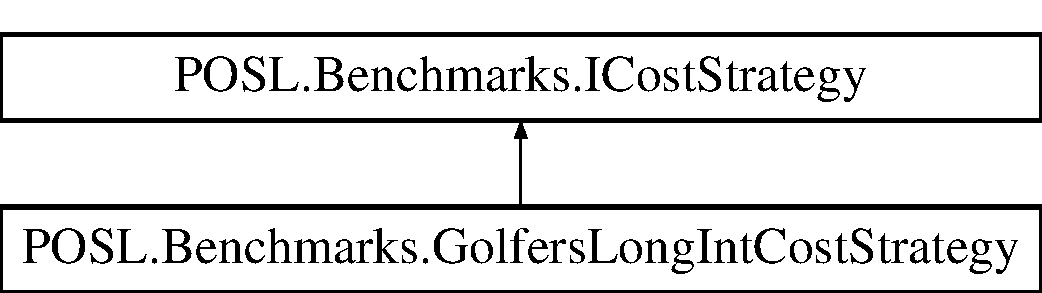
\includegraphics[height=2.000000cm]{interfacePOSL_1_1Benchmarks_1_1ICostStrategy}
\end{center}
\end{figure}
\subsection*{Public Member Functions}
\begin{DoxyCompactItemize}
\item 
int \hyperlink{interfacePOSL_1_1Benchmarks_1_1ICostStrategy_a20e3fd9e166a033eb0c395986967047f}{solution\+Cost} (\hyperlink{classPOSL_1_1Data_1_1Solution}{Solution} solution)
\begin{DoxyCompactList}\small\item\em Computes the cost of a configuration. \end{DoxyCompactList}\end{DoxyCompactItemize}


\subsection{Detailed Description}
Interface to represent an absolute solution cost strategy. 

\subsection{Member Function Documentation}
\mbox{\Hypertarget{interfacePOSL_1_1Benchmarks_1_1ICostStrategy_a20e3fd9e166a033eb0c395986967047f}\label{interfacePOSL_1_1Benchmarks_1_1ICostStrategy_a20e3fd9e166a033eb0c395986967047f}} 
\index{P\+O\+S\+L\+::\+Benchmarks\+::\+I\+Cost\+Strategy@{P\+O\+S\+L\+::\+Benchmarks\+::\+I\+Cost\+Strategy}!solution\+Cost@{solution\+Cost}}
\index{solution\+Cost@{solution\+Cost}!P\+O\+S\+L\+::\+Benchmarks\+::\+I\+Cost\+Strategy@{P\+O\+S\+L\+::\+Benchmarks\+::\+I\+Cost\+Strategy}}
\subsubsection{\texorpdfstring{solution\+Cost()}{solutionCost()}}
{\footnotesize\ttfamily int P\+O\+S\+L.\+Benchmarks.\+I\+Cost\+Strategy.\+solution\+Cost (\begin{DoxyParamCaption}\item[{\hyperlink{classPOSL_1_1Data_1_1Solution}{Solution}}]{solution }\end{DoxyParamCaption})}



Computes the cost of a configuration. 


\begin{DoxyParams}{Parameters}
{\em \+\_\+configuration} & A configuration (solution). \\
\hline
\end{DoxyParams}
\begin{DoxyReturn}{Returns}
Cost of the given configuration. 
\end{DoxyReturn}


The documentation for this class was generated from the following file\+:\begin{DoxyCompactItemize}
\item 
P\+O\+S\+L/\+P\+O\+S\+L/\+Benchmark/cost\+\_\+strategy/I\+Cost\+Strategy.\+cs\end{DoxyCompactItemize}

\hypertarget{interfacePOSL_1_1Data_1_1IDynamicNeighborhood}{}\section{P\+O\+S\+L.\+Data.\+I\+Dynamic\+Neighborhood Interface Reference}
\label{interfacePOSL_1_1Data_1_1IDynamicNeighborhood}\index{P\+O\+S\+L.\+Data.\+I\+Dynamic\+Neighborhood@{P\+O\+S\+L.\+Data.\+I\+Dynamic\+Neighborhood}}
\subsection*{Public Member Functions}
\begin{DoxyCompactItemize}
\item 
\mbox{\Hypertarget{interfacePOSL_1_1Data_1_1IDynamicNeighborhood_ae30f8372a0f40fc8a4401377c1d7e126}\label{interfacePOSL_1_1Data_1_1IDynamicNeighborhood_ae30f8372a0f40fc8a4401377c1d7e126}} 
void {\bfseries init} (\hyperlink{classPOSL_1_1Solver_1_1PSP}{P\+SP} psp, int\mbox{[}$\,$\mbox{]} \+\_\+configuration)
\end{DoxyCompactItemize}


The documentation for this interface was generated from the following file\+:\begin{DoxyCompactItemize}
\item 
P\+O\+S\+L/\+P\+O\+S\+L/\+Data/I\+Dynamic\+Neighborhood.\+cs\end{DoxyCompactItemize}

\hypertarget{interfacePOSL_1_1Data_1_1IPOSL__Iterator}{}\section{P\+O\+S\+L.\+Data.\+I\+P\+O\+S\+L\+\_\+\+Iterator Interface Reference}
\label{interfacePOSL_1_1Data_1_1IPOSL__Iterator}\index{P\+O\+S\+L.\+Data.\+I\+P\+O\+S\+L\+\_\+\+Iterator@{P\+O\+S\+L.\+Data.\+I\+P\+O\+S\+L\+\_\+\+Iterator}}
Inheritance diagram for P\+O\+S\+L.\+Data.\+I\+P\+O\+S\+L\+\_\+\+Iterator\+:\begin{figure}[H]
\begin{center}
\leavevmode
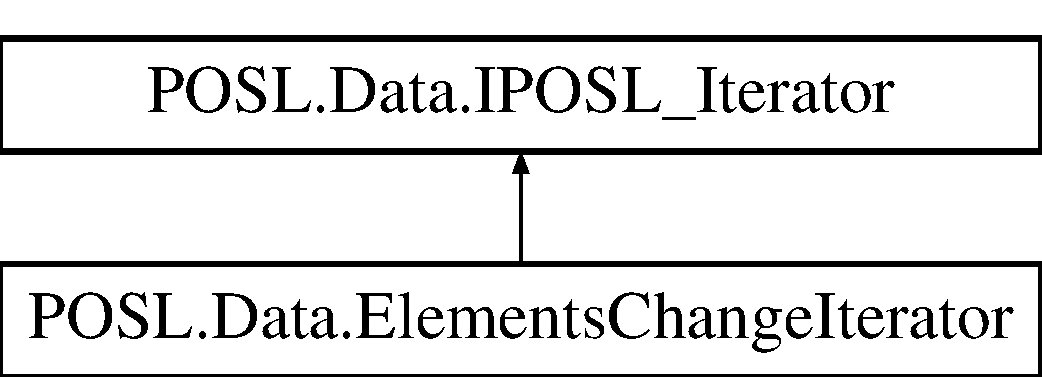
\includegraphics[height=2.000000cm]{interfacePOSL_1_1Data_1_1IPOSL__Iterator}
\end{center}
\end{figure}
\subsection*{Public Member Functions}
\begin{DoxyCompactItemize}
\item 
\mbox{\Hypertarget{interfacePOSL_1_1Data_1_1IPOSL__Iterator_a2855c33c0c7e4e8d684ea718bf19d311}\label{interfacePOSL_1_1Data_1_1IPOSL__Iterator_a2855c33c0c7e4e8d684ea718bf19d311}} 
int \mbox{[}$\,$\mbox{]} {\bfseries Get\+Next} ()
\item 
\mbox{\Hypertarget{interfacePOSL_1_1Data_1_1IPOSL__Iterator_a4df9c770cb1739c35d1f8137feb8d9fc}\label{interfacePOSL_1_1Data_1_1IPOSL__Iterator_a4df9c770cb1739c35d1f8137feb8d9fc}} 
bool {\bfseries Some\+Next} ()
\item 
\mbox{\Hypertarget{interfacePOSL_1_1Data_1_1IPOSL__Iterator_a1889fdd7b9b6b8f7029ada504a6b1c15}\label{interfacePOSL_1_1Data_1_1IPOSL__Iterator_a1889fdd7b9b6b8f7029ada504a6b1c15}} 
void {\bfseries Reset} ()
\end{DoxyCompactItemize}


The documentation for this interface was generated from the following file\+:\begin{DoxyCompactItemize}
\item 
P\+O\+S\+L/\+P\+O\+S\+L/\+Data/data\+\_\+strategy/I\+P\+O\+S\+L\+\_\+\+Iterator.\+cs\end{DoxyCompactItemize}

\hypertarget{interfacePOSL_1_1Benchmarks_1_1IProjectableCost}{}\section{P\+O\+S\+L.\+Benchmarks.\+I\+Projectable\+Cost Class Reference}
\label{interfacePOSL_1_1Benchmarks_1_1IProjectableCost}\index{P\+O\+S\+L.\+Benchmarks.\+I\+Projectable\+Cost@{P\+O\+S\+L.\+Benchmarks.\+I\+Projectable\+Cost}}


Interface to represent the a class that can projec the cost of a variable.  


\subsection*{Public Member Functions}
\begin{DoxyCompactItemize}
\item 
int \hyperlink{interfacePOSL_1_1Benchmarks_1_1IProjectableCost_a14a7025acdd7089e6fbc48a65f55487b}{cost\+On\+Variable} (int variable\+\_\+index)
\begin{DoxyCompactList}\small\item\em Computes the projected cost of a variable. \end{DoxyCompactList}\end{DoxyCompactItemize}


\subsection{Detailed Description}
Interface to represent the a class that can projec the cost of a variable. 

\subsection{Member Function Documentation}
\mbox{\Hypertarget{interfacePOSL_1_1Benchmarks_1_1IProjectableCost_a14a7025acdd7089e6fbc48a65f55487b}\label{interfacePOSL_1_1Benchmarks_1_1IProjectableCost_a14a7025acdd7089e6fbc48a65f55487b}} 
\index{P\+O\+S\+L\+::\+Benchmarks\+::\+I\+Projectable\+Cost@{P\+O\+S\+L\+::\+Benchmarks\+::\+I\+Projectable\+Cost}!cost\+On\+Variable@{cost\+On\+Variable}}
\index{cost\+On\+Variable@{cost\+On\+Variable}!P\+O\+S\+L\+::\+Benchmarks\+::\+I\+Projectable\+Cost@{P\+O\+S\+L\+::\+Benchmarks\+::\+I\+Projectable\+Cost}}
\subsubsection{\texorpdfstring{cost\+On\+Variable()}{costOnVariable()}}
{\footnotesize\ttfamily int P\+O\+S\+L.\+Benchmarks.\+I\+Projectable\+Cost.\+cost\+On\+Variable (\begin{DoxyParamCaption}\item[{int}]{variable\+\_\+index }\end{DoxyParamCaption})}



Computes the projected cost of a variable. 


\begin{DoxyParams}{Parameters}
{\em variable\+\_\+index} & Index of a variable. \\
\hline
\end{DoxyParams}
\begin{DoxyReturn}{Returns}
Projected cost of a given variable. 
\end{DoxyReturn}


The documentation for this class was generated from the following file\+:\begin{DoxyCompactItemize}
\item 
P\+O\+S\+L/\+P\+O\+S\+L/\+Benchmark/cost\+\_\+strategy/I\+Projectable\+Cost.\+cs\end{DoxyCompactItemize}

\hypertarget{interfacePOSL_1_1Benchmarks_1_1IRelativeCostStrategy}{}\section{P\+O\+S\+L.\+Benchmarks.\+I\+Relative\+Cost\+Strategy Class Reference}
\label{interfacePOSL_1_1Benchmarks_1_1IRelativeCostStrategy}\index{P\+O\+S\+L.\+Benchmarks.\+I\+Relative\+Cost\+Strategy@{P\+O\+S\+L.\+Benchmarks.\+I\+Relative\+Cost\+Strategy}}


Interface to represent a relative solution cost strategy.  


Inheritance diagram for P\+O\+S\+L.\+Benchmarks.\+I\+Relative\+Cost\+Strategy\+:\begin{figure}[H]
\begin{center}
\leavevmode
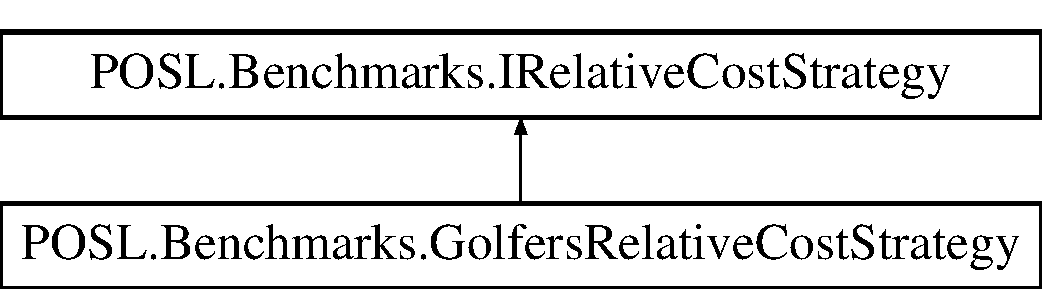
\includegraphics[height=2.000000cm]{interfacePOSL_1_1Benchmarks_1_1IRelativeCostStrategy}
\end{center}
\end{figure}
\subsection*{Public Member Functions}
\begin{DoxyCompactItemize}
\item 
int \hyperlink{interfacePOSL_1_1Benchmarks_1_1IRelativeCostStrategy_a6fe0080196e13becddbd8ff93612d9ac}{relative\+Solution\+Cost} (\hyperlink{classPOSL_1_1Data_1_1Solution}{Solution} solution)
\begin{DoxyCompactList}\small\item\em Computes the cost of a configuration relative to the current configuration. \end{DoxyCompactList}\item 
void \hyperlink{interfacePOSL_1_1Benchmarks_1_1IRelativeCostStrategy_a068a26820f0944ada9c38e30a4e4d593}{initialize\+Cost\+Data} (\hyperlink{classPOSL_1_1Data_1_1Solution}{Solution} solution, int \+\_\+initial\+\_\+cost)
\begin{DoxyCompactList}\small\item\em Initialize the information related to the cost. \end{DoxyCompactList}\item 
int \hyperlink{interfacePOSL_1_1Benchmarks_1_1IRelativeCostStrategy_a4582db712ef4cbb67b790459f7c441ac}{relative\+Solution\+Cost} (\hyperlink{classPOSL_1_1Data_1_1Solution}{Solution} solution, \hyperlink{structPOSL_1_1Tools_1_1T__Changes}{T\+\_\+\+Changes} \+\_\+change)
\begin{DoxyCompactList}\small\item\em Computes the cost of a configuration relative to the current configuration. \end{DoxyCompactList}\item 
void \hyperlink{interfacePOSL_1_1Benchmarks_1_1IRelativeCostStrategy_a74e16251c8b6304dec763e640e19f1df}{update\+Configuration} (\hyperlink{classPOSL_1_1Data_1_1Solution}{Solution} new\+\_\+solution)
\begin{DoxyCompactList}\small\item\em Updates the current configuration. \end{DoxyCompactList}\item 
int \hyperlink{interfacePOSL_1_1Benchmarks_1_1IRelativeCostStrategy_a98945d070a021b588b10f79ca3ea8f4b}{current\+Cost} ()
\begin{DoxyCompactList}\small\item\em Returns the current cost. \end{DoxyCompactList}\item 
int \hyperlink{interfacePOSL_1_1Benchmarks_1_1IRelativeCostStrategy_aab0193ee08a9bbe6648c1b8f6db0556a}{cost\+On\+Variable} (int variable\+\_\+index)
\begin{DoxyCompactList}\small\item\em Computes the projected cost of a variable. \end{DoxyCompactList}\item 
int \hyperlink{interfacePOSL_1_1Benchmarks_1_1IRelativeCostStrategy_ae52e1ef62b902b5e87be5f6bcdb64dbc}{sickest\+Variable} ()
\begin{DoxyCompactList}\small\item\em Returns the variable with the highest projected cost. \end{DoxyCompactList}\end{DoxyCompactItemize}


\subsection{Detailed Description}
Interface to represent a relative solution cost strategy. 

\subsection{Member Function Documentation}
\mbox{\Hypertarget{interfacePOSL_1_1Benchmarks_1_1IRelativeCostStrategy_aab0193ee08a9bbe6648c1b8f6db0556a}\label{interfacePOSL_1_1Benchmarks_1_1IRelativeCostStrategy_aab0193ee08a9bbe6648c1b8f6db0556a}} 
\index{P\+O\+S\+L\+::\+Benchmarks\+::\+I\+Relative\+Cost\+Strategy@{P\+O\+S\+L\+::\+Benchmarks\+::\+I\+Relative\+Cost\+Strategy}!cost\+On\+Variable@{cost\+On\+Variable}}
\index{cost\+On\+Variable@{cost\+On\+Variable}!P\+O\+S\+L\+::\+Benchmarks\+::\+I\+Relative\+Cost\+Strategy@{P\+O\+S\+L\+::\+Benchmarks\+::\+I\+Relative\+Cost\+Strategy}}
\subsubsection{\texorpdfstring{cost\+On\+Variable()}{costOnVariable()}}
{\footnotesize\ttfamily int P\+O\+S\+L.\+Benchmarks.\+I\+Relative\+Cost\+Strategy.\+cost\+On\+Variable (\begin{DoxyParamCaption}\item[{int}]{variable\+\_\+index }\end{DoxyParamCaption})}



Computes the projected cost of a variable. 


\begin{DoxyParams}{Parameters}
{\em variable\+\_\+index} & Index of a variable. \\
\hline
\end{DoxyParams}
\begin{DoxyReturn}{Returns}
The projected cost of the variable with index {\itshape variable\+\_\+index}. 
\end{DoxyReturn}
\mbox{\Hypertarget{interfacePOSL_1_1Benchmarks_1_1IRelativeCostStrategy_a98945d070a021b588b10f79ca3ea8f4b}\label{interfacePOSL_1_1Benchmarks_1_1IRelativeCostStrategy_a98945d070a021b588b10f79ca3ea8f4b}} 
\index{P\+O\+S\+L\+::\+Benchmarks\+::\+I\+Relative\+Cost\+Strategy@{P\+O\+S\+L\+::\+Benchmarks\+::\+I\+Relative\+Cost\+Strategy}!current\+Cost@{current\+Cost}}
\index{current\+Cost@{current\+Cost}!P\+O\+S\+L\+::\+Benchmarks\+::\+I\+Relative\+Cost\+Strategy@{P\+O\+S\+L\+::\+Benchmarks\+::\+I\+Relative\+Cost\+Strategy}}
\subsubsection{\texorpdfstring{current\+Cost()}{currentCost()}}
{\footnotesize\ttfamily int P\+O\+S\+L.\+Benchmarks.\+I\+Relative\+Cost\+Strategy.\+current\+Cost (\begin{DoxyParamCaption}{ }\end{DoxyParamCaption})}



Returns the current cost. 

\begin{DoxyReturn}{Returns}
Current cost. 
\end{DoxyReturn}
\mbox{\Hypertarget{interfacePOSL_1_1Benchmarks_1_1IRelativeCostStrategy_a068a26820f0944ada9c38e30a4e4d593}\label{interfacePOSL_1_1Benchmarks_1_1IRelativeCostStrategy_a068a26820f0944ada9c38e30a4e4d593}} 
\index{P\+O\+S\+L\+::\+Benchmarks\+::\+I\+Relative\+Cost\+Strategy@{P\+O\+S\+L\+::\+Benchmarks\+::\+I\+Relative\+Cost\+Strategy}!initialize\+Cost\+Data@{initialize\+Cost\+Data}}
\index{initialize\+Cost\+Data@{initialize\+Cost\+Data}!P\+O\+S\+L\+::\+Benchmarks\+::\+I\+Relative\+Cost\+Strategy@{P\+O\+S\+L\+::\+Benchmarks\+::\+I\+Relative\+Cost\+Strategy}}
\subsubsection{\texorpdfstring{initialize\+Cost\+Data()}{initializeCostData()}}
{\footnotesize\ttfamily void P\+O\+S\+L.\+Benchmarks.\+I\+Relative\+Cost\+Strategy.\+initialize\+Cost\+Data (\begin{DoxyParamCaption}\item[{\hyperlink{classPOSL_1_1Data_1_1Solution}{Solution}}]{solution,  }\item[{int}]{\+\_\+initial\+\_\+cost }\end{DoxyParamCaption})}



Initialize the information related to the cost. 


\begin{DoxyParams}{Parameters}
{\em \+\_\+configuration} & A configuration (solution). \\
\hline
{\em \+\_\+initial\+\_\+cost} & The initial cost of the configuration. \\
\hline
\end{DoxyParams}
\mbox{\Hypertarget{interfacePOSL_1_1Benchmarks_1_1IRelativeCostStrategy_a6fe0080196e13becddbd8ff93612d9ac}\label{interfacePOSL_1_1Benchmarks_1_1IRelativeCostStrategy_a6fe0080196e13becddbd8ff93612d9ac}} 
\index{P\+O\+S\+L\+::\+Benchmarks\+::\+I\+Relative\+Cost\+Strategy@{P\+O\+S\+L\+::\+Benchmarks\+::\+I\+Relative\+Cost\+Strategy}!relative\+Solution\+Cost@{relative\+Solution\+Cost}}
\index{relative\+Solution\+Cost@{relative\+Solution\+Cost}!P\+O\+S\+L\+::\+Benchmarks\+::\+I\+Relative\+Cost\+Strategy@{P\+O\+S\+L\+::\+Benchmarks\+::\+I\+Relative\+Cost\+Strategy}}
\subsubsection{\texorpdfstring{relative\+Solution\+Cost()}{relativeSolutionCost()}\hspace{0.1cm}{\footnotesize\ttfamily [1/2]}}
{\footnotesize\ttfamily int P\+O\+S\+L.\+Benchmarks.\+I\+Relative\+Cost\+Strategy.\+relative\+Solution\+Cost (\begin{DoxyParamCaption}\item[{\hyperlink{classPOSL_1_1Data_1_1Solution}{Solution}}]{solution }\end{DoxyParamCaption})}



Computes the cost of a configuration relative to the current configuration. 


\begin{DoxyParams}{Parameters}
{\em solution} & A configuration (solution). \\
\hline
\end{DoxyParams}
\begin{DoxyReturn}{Returns}
Cost of the given configuration. 
\end{DoxyReturn}
\mbox{\Hypertarget{interfacePOSL_1_1Benchmarks_1_1IRelativeCostStrategy_a4582db712ef4cbb67b790459f7c441ac}\label{interfacePOSL_1_1Benchmarks_1_1IRelativeCostStrategy_a4582db712ef4cbb67b790459f7c441ac}} 
\index{P\+O\+S\+L\+::\+Benchmarks\+::\+I\+Relative\+Cost\+Strategy@{P\+O\+S\+L\+::\+Benchmarks\+::\+I\+Relative\+Cost\+Strategy}!relative\+Solution\+Cost@{relative\+Solution\+Cost}}
\index{relative\+Solution\+Cost@{relative\+Solution\+Cost}!P\+O\+S\+L\+::\+Benchmarks\+::\+I\+Relative\+Cost\+Strategy@{P\+O\+S\+L\+::\+Benchmarks\+::\+I\+Relative\+Cost\+Strategy}}
\subsubsection{\texorpdfstring{relative\+Solution\+Cost()}{relativeSolutionCost()}\hspace{0.1cm}{\footnotesize\ttfamily [2/2]}}
{\footnotesize\ttfamily int P\+O\+S\+L.\+Benchmarks.\+I\+Relative\+Cost\+Strategy.\+relative\+Solution\+Cost (\begin{DoxyParamCaption}\item[{\hyperlink{classPOSL_1_1Data_1_1Solution}{Solution}}]{solution,  }\item[{\hyperlink{structPOSL_1_1Tools_1_1T__Changes}{T\+\_\+\+Changes}}]{\+\_\+change }\end{DoxyParamCaption})}



Computes the cost of a configuration relative to the current configuration. 


\begin{DoxyParams}{Parameters}
{\em \+\_\+configuration} & A configuration (solution). \\
\hline
{\em \+\_\+change} & The performed changes w.\+r.\+t the current configuration \\
\hline
\end{DoxyParams}
\begin{DoxyReturn}{Returns}
Cost of the given configuration. 
\end{DoxyReturn}
\mbox{\Hypertarget{interfacePOSL_1_1Benchmarks_1_1IRelativeCostStrategy_ae52e1ef62b902b5e87be5f6bcdb64dbc}\label{interfacePOSL_1_1Benchmarks_1_1IRelativeCostStrategy_ae52e1ef62b902b5e87be5f6bcdb64dbc}} 
\index{P\+O\+S\+L\+::\+Benchmarks\+::\+I\+Relative\+Cost\+Strategy@{P\+O\+S\+L\+::\+Benchmarks\+::\+I\+Relative\+Cost\+Strategy}!sickest\+Variable@{sickest\+Variable}}
\index{sickest\+Variable@{sickest\+Variable}!P\+O\+S\+L\+::\+Benchmarks\+::\+I\+Relative\+Cost\+Strategy@{P\+O\+S\+L\+::\+Benchmarks\+::\+I\+Relative\+Cost\+Strategy}}
\subsubsection{\texorpdfstring{sickest\+Variable()}{sickestVariable()}}
{\footnotesize\ttfamily int P\+O\+S\+L.\+Benchmarks.\+I\+Relative\+Cost\+Strategy.\+sickest\+Variable (\begin{DoxyParamCaption}{ }\end{DoxyParamCaption})}



Returns the variable with the highest projected cost. 

\begin{DoxyReturn}{Returns}
The projected cost of the variable with highest projected cost. 
\end{DoxyReturn}
\mbox{\Hypertarget{interfacePOSL_1_1Benchmarks_1_1IRelativeCostStrategy_a74e16251c8b6304dec763e640e19f1df}\label{interfacePOSL_1_1Benchmarks_1_1IRelativeCostStrategy_a74e16251c8b6304dec763e640e19f1df}} 
\index{P\+O\+S\+L\+::\+Benchmarks\+::\+I\+Relative\+Cost\+Strategy@{P\+O\+S\+L\+::\+Benchmarks\+::\+I\+Relative\+Cost\+Strategy}!update\+Configuration@{update\+Configuration}}
\index{update\+Configuration@{update\+Configuration}!P\+O\+S\+L\+::\+Benchmarks\+::\+I\+Relative\+Cost\+Strategy@{P\+O\+S\+L\+::\+Benchmarks\+::\+I\+Relative\+Cost\+Strategy}}
\subsubsection{\texorpdfstring{update\+Configuration()}{updateConfiguration()}}
{\footnotesize\ttfamily void P\+O\+S\+L.\+Benchmarks.\+I\+Relative\+Cost\+Strategy.\+update\+Configuration (\begin{DoxyParamCaption}\item[{\hyperlink{classPOSL_1_1Data_1_1Solution}{Solution}}]{new\+\_\+solution }\end{DoxyParamCaption})}



Updates the current configuration. 


\begin{DoxyParams}{Parameters}
{\em new\+\_\+config} & A configuration (solution). \\
\hline
\end{DoxyParams}


The documentation for this class was generated from the following file\+:\begin{DoxyCompactItemize}
\item 
P\+O\+S\+L/\+P\+O\+S\+L/\+Benchmark/cost\+\_\+strategy/I\+Relative\+Cost\+Strategy.\+cs\end{DoxyCompactItemize}

\hypertarget{interfacePOSL_1_1Benchmarks_1_1IReseteable}{}\section{P\+O\+S\+L.\+Benchmarks.\+I\+Reseteable Class Reference}
\label{interfacePOSL_1_1Benchmarks_1_1IReseteable}\index{P\+O\+S\+L.\+Benchmarks.\+I\+Reseteable@{P\+O\+S\+L.\+Benchmarks.\+I\+Reseteable}}


Interface to represent a relative solution cost strategy.  


\subsection*{Public Member Functions}
\begin{DoxyCompactItemize}
\item 
int \mbox{[}$\,$\mbox{]} \hyperlink{interfacePOSL_1_1Benchmarks_1_1IReseteable_a79beca76a4dd94b2543aa34d8c0adbc9}{reset} ()
\begin{DoxyCompactList}\small\item\em Performs a reset w.\+r.\+t. the current configuration. \end{DoxyCompactList}\end{DoxyCompactItemize}


\subsection{Detailed Description}
Interface to represent a relative solution cost strategy. 

\subsection{Member Function Documentation}
\mbox{\Hypertarget{interfacePOSL_1_1Benchmarks_1_1IReseteable_a79beca76a4dd94b2543aa34d8c0adbc9}\label{interfacePOSL_1_1Benchmarks_1_1IReseteable_a79beca76a4dd94b2543aa34d8c0adbc9}} 
\index{P\+O\+S\+L\+::\+Benchmarks\+::\+I\+Reseteable@{P\+O\+S\+L\+::\+Benchmarks\+::\+I\+Reseteable}!reset@{reset}}
\index{reset@{reset}!P\+O\+S\+L\+::\+Benchmarks\+::\+I\+Reseteable@{P\+O\+S\+L\+::\+Benchmarks\+::\+I\+Reseteable}}
\subsubsection{\texorpdfstring{reset()}{reset()}}
{\footnotesize\ttfamily int \mbox{[}$\,$\mbox{]} P\+O\+S\+L.\+Benchmarks.\+I\+Reseteable.\+reset (\begin{DoxyParamCaption}{ }\end{DoxyParamCaption})}



Performs a reset w.\+r.\+t. the current configuration. 

\begin{DoxyReturn}{Returns}
A {\itshape reseted} configuration. 
\end{DoxyReturn}


The documentation for this class was generated from the following file\+:\begin{DoxyCompactItemize}
\item 
P\+O\+S\+L/\+P\+O\+S\+L/\+Benchmark/cost\+\_\+strategy/I\+Reseteable.\+cs\end{DoxyCompactItemize}

\hypertarget{interfacePOSL_1_1Benchmarks_1_1IShowStrategy}{}\section{P\+O\+S\+L.\+Benchmarks.\+I\+Show\+Strategy Class Reference}
\label{interfacePOSL_1_1Benchmarks_1_1IShowStrategy}\index{P\+O\+S\+L.\+Benchmarks.\+I\+Show\+Strategy@{P\+O\+S\+L.\+Benchmarks.\+I\+Show\+Strategy}}


Interface to represent the way a problem shows its result (solution)  


Inheritance diagram for P\+O\+S\+L.\+Benchmarks.\+I\+Show\+Strategy\+:\begin{figure}[H]
\begin{center}
\leavevmode
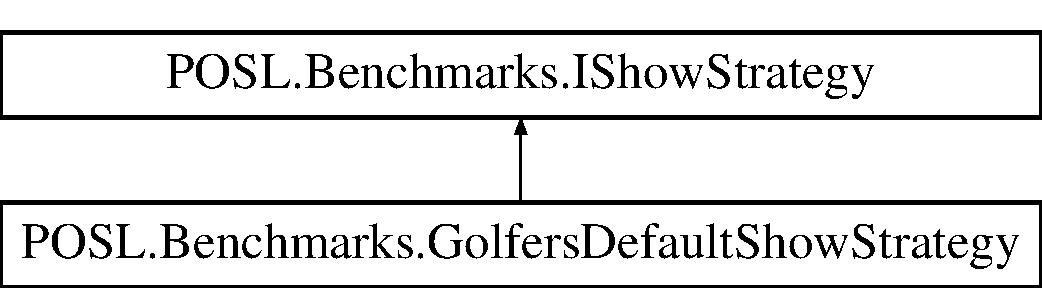
\includegraphics[height=2.000000cm]{interfacePOSL_1_1Benchmarks_1_1IShowStrategy}
\end{center}
\end{figure}
\subsection*{Public Member Functions}
\begin{DoxyCompactItemize}
\item 
string \hyperlink{interfacePOSL_1_1Benchmarks_1_1IShowStrategy_afee02368af80da9bc782bb0ec1e72844}{show\+Solution} (\hyperlink{classPOSL_1_1Data_1_1Solution}{Solution} solution)
\begin{DoxyCompactList}\small\item\em Default constructor. \end{DoxyCompactList}\end{DoxyCompactItemize}


\subsection{Detailed Description}
Interface to represent the way a problem shows its result (solution) 

\subsection{Member Function Documentation}
\mbox{\Hypertarget{interfacePOSL_1_1Benchmarks_1_1IShowStrategy_afee02368af80da9bc782bb0ec1e72844}\label{interfacePOSL_1_1Benchmarks_1_1IShowStrategy_afee02368af80da9bc782bb0ec1e72844}} 
\index{P\+O\+S\+L\+::\+Benchmarks\+::\+I\+Show\+Strategy@{P\+O\+S\+L\+::\+Benchmarks\+::\+I\+Show\+Strategy}!show\+Solution@{show\+Solution}}
\index{show\+Solution@{show\+Solution}!P\+O\+S\+L\+::\+Benchmarks\+::\+I\+Show\+Strategy@{P\+O\+S\+L\+::\+Benchmarks\+::\+I\+Show\+Strategy}}
\subsubsection{\texorpdfstring{show\+Solution()}{showSolution()}}
{\footnotesize\ttfamily string P\+O\+S\+L.\+Benchmarks.\+I\+Show\+Strategy.\+show\+Solution (\begin{DoxyParamCaption}\item[{\hyperlink{classPOSL_1_1Data_1_1Solution}{Solution}}]{solution }\end{DoxyParamCaption})}



Default constructor. 


\begin{DoxyParams}{Parameters}
{\em solution} & A solution to some problem. \\
\hline
\end{DoxyParams}
\begin{DoxyReturn}{Returns}
String to show 
\end{DoxyReturn}


The documentation for this class was generated from the following file\+:\begin{DoxyCompactItemize}
\item 
P\+O\+S\+L/\+P\+O\+S\+L/\+Benchmark/showing\+\_\+strategy/I\+Show\+Strategy.\+cs\end{DoxyCompactItemize}

\hypertarget{interfacePOSL_1_1Benchmarks_1_1ISickestVariableStrategy}{}\section{P\+O\+S\+L.\+Benchmarks.\+I\+Sickest\+Variable\+Strategy Class Reference}
\label{interfacePOSL_1_1Benchmarks_1_1ISickestVariableStrategy}\index{P\+O\+S\+L.\+Benchmarks.\+I\+Sickest\+Variable\+Strategy@{P\+O\+S\+L.\+Benchmarks.\+I\+Sickest\+Variable\+Strategy}}


Interface to represent a strategy to compute the variable with the highest projected cost.  


\subsection*{Public Member Functions}
\begin{DoxyCompactItemize}
\item 
int \hyperlink{interfacePOSL_1_1Benchmarks_1_1ISickestVariableStrategy_a32b331ff755030c8404e2a0a174c6bcd}{sickest\+Variable} ()
\begin{DoxyCompactList}\small\item\em Returns the variable with the highest projected cost. \end{DoxyCompactList}\end{DoxyCompactItemize}


\subsection{Detailed Description}
Interface to represent a strategy to compute the variable with the highest projected cost. 

\subsection{Member Function Documentation}
\mbox{\Hypertarget{interfacePOSL_1_1Benchmarks_1_1ISickestVariableStrategy_a32b331ff755030c8404e2a0a174c6bcd}\label{interfacePOSL_1_1Benchmarks_1_1ISickestVariableStrategy_a32b331ff755030c8404e2a0a174c6bcd}} 
\index{P\+O\+S\+L\+::\+Benchmarks\+::\+I\+Sickest\+Variable\+Strategy@{P\+O\+S\+L\+::\+Benchmarks\+::\+I\+Sickest\+Variable\+Strategy}!sickest\+Variable@{sickest\+Variable}}
\index{sickest\+Variable@{sickest\+Variable}!P\+O\+S\+L\+::\+Benchmarks\+::\+I\+Sickest\+Variable\+Strategy@{P\+O\+S\+L\+::\+Benchmarks\+::\+I\+Sickest\+Variable\+Strategy}}
\subsubsection{\texorpdfstring{sickest\+Variable()}{sickestVariable()}}
{\footnotesize\ttfamily int P\+O\+S\+L.\+Benchmarks.\+I\+Sickest\+Variable\+Strategy.\+sickest\+Variable (\begin{DoxyParamCaption}{ }\end{DoxyParamCaption})}



Returns the variable with the highest projected cost. 

\begin{DoxyReturn}{Returns}
The index of the variable with the highest projected cost. 
\end{DoxyReturn}


The documentation for this class was generated from the following file\+:\begin{DoxyCompactItemize}
\item 
P\+O\+S\+L/\+P\+O\+S\+L/\+Benchmark/cost\+\_\+strategy/I\+Sickest\+Variable\+Strategy.\+cs\end{DoxyCompactItemize}

\hypertarget{classPOSL_1_1Tools_1_1LongInt}{}\section{P\+O\+S\+L.\+Tools.\+Long\+Int Class Reference}
\label{classPOSL_1_1Tools_1_1LongInt}\index{P\+O\+S\+L.\+Tools.\+Long\+Int@{P\+O\+S\+L.\+Tools.\+Long\+Int}}
\subsection*{Public Member Functions}
\begin{DoxyCompactItemize}
\item 
\mbox{\Hypertarget{classPOSL_1_1Tools_1_1LongInt_ac760ee8fc21b9624229255fc27698903}\label{classPOSL_1_1Tools_1_1LongInt_ac760ee8fc21b9624229255fc27698903}} 
{\bfseries Long\+Int} (int \+\_\+bytes, int\mbox{[}$\,$\mbox{]} \+\_\+value)
\item 
\mbox{\Hypertarget{classPOSL_1_1Tools_1_1LongInt_a52106799c2af1366abbecd6fe1fd1272}\label{classPOSL_1_1Tools_1_1LongInt_a52106799c2af1366abbecd6fe1fd1272}} 
{\bfseries Long\+Int} (int \+\_\+bytes, int \+\_\+value)
\item 
\mbox{\Hypertarget{classPOSL_1_1Tools_1_1LongInt_a6ca4833858e9cc3a60629aadefc1f041}\label{classPOSL_1_1Tools_1_1LongInt_a6ca4833858e9cc3a60629aadefc1f041}} 
{\bfseries Long\+Int} (int \+\_\+bytes)
\item 
\mbox{\Hypertarget{classPOSL_1_1Tools_1_1LongInt_aa1ad5c9aee846670b7af608a397675b9}\label{classPOSL_1_1Tools_1_1LongInt_aa1ad5c9aee846670b7af608a397675b9}} 
bool {\bfseries activated} ()
\item 
\mbox{\Hypertarget{classPOSL_1_1Tools_1_1LongInt_add69f1fe0606fb43a26247ce8a66d2fc}\label{classPOSL_1_1Tools_1_1LongInt_add69f1fe0606fb43a26247ce8a66d2fc}} 
bool {\bfseries activated} (int bit)
\item 
\mbox{\Hypertarget{classPOSL_1_1Tools_1_1LongInt_a7924ccf65097b41d50640722268b1124}\label{classPOSL_1_1Tools_1_1LongInt_a7924ccf65097b41d50640722268b1124}} 
void {\bfseries activate} (int bit)
\item 
\mbox{\Hypertarget{classPOSL_1_1Tools_1_1LongInt_ad2eecb88d41d6887b0958973a7364d39}\label{classPOSL_1_1Tools_1_1LongInt_ad2eecb88d41d6887b0958973a7364d39}} 
void {\bfseries activate\+All} ()
\item 
\mbox{\Hypertarget{classPOSL_1_1Tools_1_1LongInt_ad8b23ce2d91ab32a676403666bb195d5}\label{classPOSL_1_1Tools_1_1LongInt_ad8b23ce2d91ab32a676403666bb195d5}} 
void {\bfseries deactivate\+All} ()
\item 
\mbox{\Hypertarget{classPOSL_1_1Tools_1_1LongInt_a5249a8142bf430fb034e10d953e1cdb7}\label{classPOSL_1_1Tools_1_1LongInt_a5249a8142bf430fb034e10d953e1cdb7}} 
int {\bfseries bit\+Count} ()
\item 
\mbox{\Hypertarget{classPOSL_1_1Tools_1_1LongInt_a20d07c89e9e5c1b43adb7ef595df9ba2}\label{classPOSL_1_1Tools_1_1LongInt_a20d07c89e9e5c1b43adb7ef595df9ba2}} 
bool {\bfseries Equal} (\hyperlink{classPOSL_1_1Tools_1_1LongInt}{Long\+Int} other)
\item 
\mbox{\Hypertarget{classPOSL_1_1Tools_1_1LongInt_a549c0bf554df2994e3d02048efc306f1}\label{classPOSL_1_1Tools_1_1LongInt_a549c0bf554df2994e3d02048efc306f1}} 
string {\bfseries binary} (int val, int bit)
\item 
\mbox{\Hypertarget{classPOSL_1_1Tools_1_1LongInt_ae71c42d1e8c99aac66089ddf039133c7}\label{classPOSL_1_1Tools_1_1LongInt_ae71c42d1e8c99aac66089ddf039133c7}} 
string {\bfseries to\+String} ()
\end{DoxyCompactItemize}
\subsection*{Static Public Member Functions}
\begin{DoxyCompactItemize}
\item 
\mbox{\Hypertarget{classPOSL_1_1Tools_1_1LongInt_a59a05285b8a0ac2b680989e8a49e7db7}\label{classPOSL_1_1Tools_1_1LongInt_a59a05285b8a0ac2b680989e8a49e7db7}} 
static \hyperlink{classPOSL_1_1Tools_1_1LongInt}{Long\+Int} {\bfseries operator$\vert$} (\hyperlink{classPOSL_1_1Tools_1_1LongInt}{Long\+Int} a, \hyperlink{classPOSL_1_1Tools_1_1LongInt}{Long\+Int} b)
\item 
\mbox{\Hypertarget{classPOSL_1_1Tools_1_1LongInt_a9a85a5d9acbdb9b96cbdfcb479c787ed}\label{classPOSL_1_1Tools_1_1LongInt_a9a85a5d9acbdb9b96cbdfcb479c787ed}} 
static \hyperlink{classPOSL_1_1Tools_1_1LongInt}{Long\+Int} {\bfseries operator\&} (\hyperlink{classPOSL_1_1Tools_1_1LongInt}{Long\+Int} a, \hyperlink{classPOSL_1_1Tools_1_1LongInt}{Long\+Int} b)
\end{DoxyCompactItemize}
\subsection*{Properties}
\begin{DoxyCompactItemize}
\item 
\mbox{\Hypertarget{classPOSL_1_1Tools_1_1LongInt_a9fa7492f38b945f25e677400cd30cb53}\label{classPOSL_1_1Tools_1_1LongInt_a9fa7492f38b945f25e677400cd30cb53}} 
int {\bfseries Length}\hspace{0.3cm}{\ttfamily  \mbox{[}get\mbox{]}}
\item 
\mbox{\Hypertarget{classPOSL_1_1Tools_1_1LongInt_a1aa896fb7636d73971a58c8a673675b0}\label{classPOSL_1_1Tools_1_1LongInt_a1aa896fb7636d73971a58c8a673675b0}} 
int {\bfseries this\mbox{[}int index\mbox{]}}\hspace{0.3cm}{\ttfamily  \mbox{[}get\mbox{]}}
\end{DoxyCompactItemize}


The documentation for this class was generated from the following file\+:\begin{DoxyCompactItemize}
\item 
P\+O\+S\+L/\+P\+O\+S\+L/\+Tools/Long\+Int.\+cs\end{DoxyCompactItemize}

\hypertarget{classPOSL_1_1Tools_1_1MergedLongInt}{}\section{P\+O\+S\+L.\+Tools.\+Merged\+Long\+Int Class Reference}
\label{classPOSL_1_1Tools_1_1MergedLongInt}\index{P\+O\+S\+L.\+Tools.\+Merged\+Long\+Int@{P\+O\+S\+L.\+Tools.\+Merged\+Long\+Int}}
\subsection*{Public Member Functions}
\begin{DoxyCompactItemize}
\item 
\mbox{\Hypertarget{classPOSL_1_1Tools_1_1MergedLongInt_a6cdab3ec6127896daedcff94924458b6}\label{classPOSL_1_1Tools_1_1MergedLongInt_a6cdab3ec6127896daedcff94924458b6}} 
{\bfseries Merged\+Long\+Int} (\hyperlink{classPOSL_1_1Tools_1_1LongInt}{Long\+Int} a, \hyperlink{classPOSL_1_1Tools_1_1LongInt}{Long\+Int} b)
\item 
\mbox{\Hypertarget{classPOSL_1_1Tools_1_1MergedLongInt_a77ab115b2e737b5e9aa529af4044288e}\label{classPOSL_1_1Tools_1_1MergedLongInt_a77ab115b2e737b5e9aa529af4044288e}} 
\hyperlink{classPOSL_1_1Tools_1_1LongInt}{Long\+Int} {\bfseries long\+\_\+or} ()
\item 
\mbox{\Hypertarget{classPOSL_1_1Tools_1_1MergedLongInt_a543d8d87cdf103243867254b521773f7}\label{classPOSL_1_1Tools_1_1MergedLongInt_a543d8d87cdf103243867254b521773f7}} 
\hyperlink{classPOSL_1_1Tools_1_1LongInt}{Long\+Int} {\bfseries long\+\_\+and} ()
\item 
\mbox{\Hypertarget{classPOSL_1_1Tools_1_1MergedLongInt_a3b6ce587c0f502e9d4ef7d28066027c9}\label{classPOSL_1_1Tools_1_1MergedLongInt_a3b6ce587c0f502e9d4ef7d28066027c9}} 
bool {\bfseries equal} ()
\end{DoxyCompactItemize}


The documentation for this class was generated from the following file\+:\begin{DoxyCompactItemize}
\item 
P\+O\+S\+L/\+P\+O\+S\+L/\+Tools/Merged\+Long\+Int.\+cs\end{DoxyCompactItemize}

\hypertarget{classPOSL_1_1Data_1_1Neighborhood}{}\section{P\+O\+S\+L.\+Data.\+Neighborhood Class Reference}
\label{classPOSL_1_1Data_1_1Neighborhood}\index{P\+O\+S\+L.\+Data.\+Neighborhood@{P\+O\+S\+L.\+Data.\+Neighborhood}}


(Abstract) Class to represent a neighborhood of a configuration  


Inheritance diagram for P\+O\+S\+L.\+Data.\+Neighborhood\+:\begin{figure}[H]
\begin{center}
\leavevmode
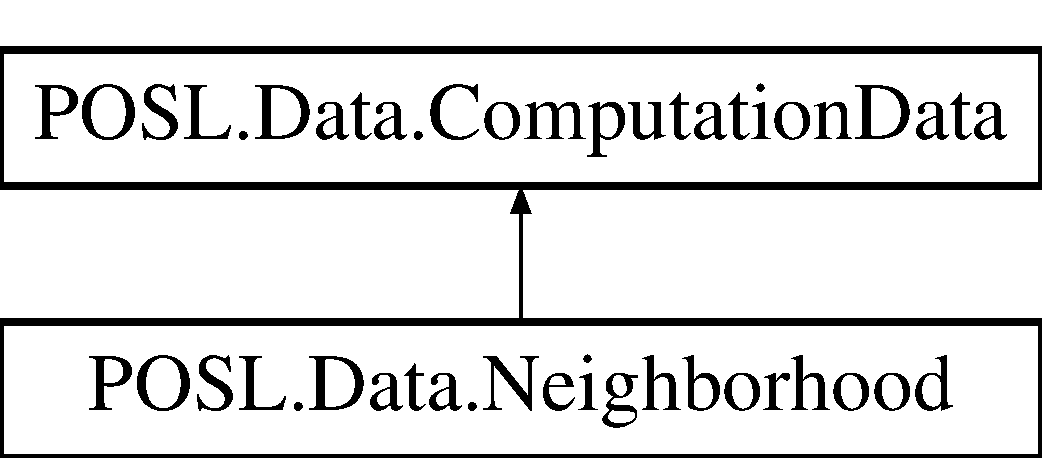
\includegraphics[height=2.000000cm]{classPOSL_1_1Data_1_1Neighborhood}
\end{center}
\end{figure}
\subsection*{Public Member Functions}
\begin{DoxyCompactItemize}
\item 
\mbox{\Hypertarget{classPOSL_1_1Data_1_1Neighborhood_a360ba755eb5e9d86a56723bb478ab469}\label{classPOSL_1_1Data_1_1Neighborhood_a360ba755eb5e9d86a56723bb478ab469}} 
{\bfseries Neighborhood} (int\mbox{[}$\,$\mbox{]} \+\_\+current\+\_\+configuration)
\item 
\mbox{\Hypertarget{classPOSL_1_1Data_1_1Neighborhood_a06bd81429e435cc7c434b29d62b8f50d}\label{classPOSL_1_1Data_1_1Neighborhood_a06bd81429e435cc7c434b29d62b8f50d}} 
{\bfseries Neighborhood} (int \+\_\+config\+\_\+size)
\item 
\mbox{\Hypertarget{classPOSL_1_1Data_1_1Neighborhood_a74e095bec02148e5816c8e11eacba9d5}\label{classPOSL_1_1Data_1_1Neighborhood_a74e095bec02148e5816c8e11eacba9d5}} 
override string {\bfseries Tag} ()
\item 
override int \hyperlink{classPOSL_1_1Data_1_1Neighborhood_aa7014a3cbaf532f49d89468c20b7c269}{comapare\+To} (\hyperlink{classPOSL_1_1Data_1_1ComputationData}{Computation\+Data} other, Func$<$ \hyperlink{classPOSL_1_1Data_1_1ComputationData}{Computation\+Data}, int $>$ criteria)
\begin{DoxyCompactList}\small\item\em Compare this object with other, given a function (criteria) \end{DoxyCompactList}\item 
\mbox{\Hypertarget{classPOSL_1_1Data_1_1Neighborhood_a3bf4058bac77b7a30623de0621536cb3}\label{classPOSL_1_1Data_1_1Neighborhood_a3bf4058bac77b7a30623de0621536cb3}} 
abstract \hyperlink{interfacePOSL_1_1Data_1_1IPOSL__Iterator}{I\+P\+O\+S\+L\+\_\+\+Iterator} {\bfseries get\+Iterator} ()
\end{DoxyCompactItemize}
\subsection*{Properties}
\begin{DoxyCompactItemize}
\item 
\mbox{\Hypertarget{classPOSL_1_1Data_1_1Neighborhood_a3f456c4d9b95e61ad17e3c68f5a1930e}\label{classPOSL_1_1Data_1_1Neighborhood_a3f456c4d9b95e61ad17e3c68f5a1930e}} 
int \mbox{[}$\,$\mbox{]} {\bfseries Current\+Configuration}\hspace{0.3cm}{\ttfamily  \mbox{[}get\mbox{]}}
\item 
\mbox{\Hypertarget{classPOSL_1_1Data_1_1Neighborhood_a7363f3e9bb33274139142cb36292b816}\label{classPOSL_1_1Data_1_1Neighborhood_a7363f3e9bb33274139142cb36292b816}} 
string {\bfseries Solution\+Packing\+ID}\hspace{0.3cm}{\ttfamily  \mbox{[}get\mbox{]}}
\item 
\mbox{\Hypertarget{classPOSL_1_1Data_1_1Neighborhood_a1b9d521ea7bf517c33a513215ef65582}\label{classPOSL_1_1Data_1_1Neighborhood_a1b9d521ea7bf517c33a513215ef65582}} 
abstract int {\bfseries Size}\hspace{0.3cm}{\ttfamily  \mbox{[}get\mbox{]}}
\item 
\mbox{\Hypertarget{classPOSL_1_1Data_1_1Neighborhood_a492cc83da8bb5955f5dc42a14d4423ec}\label{classPOSL_1_1Data_1_1Neighborhood_a492cc83da8bb5955f5dc42a14d4423ec}} 
abstract int \mbox{[}$\,$\mbox{]} {\bfseries this\mbox{[}int index\mbox{]}}\hspace{0.3cm}{\ttfamily  \mbox{[}get\mbox{]}}
\end{DoxyCompactItemize}


\subsection{Detailed Description}
(Abstract) Class to represent a neighborhood of a configuration 

\subsection{Member Function Documentation}
\mbox{\Hypertarget{classPOSL_1_1Data_1_1Neighborhood_aa7014a3cbaf532f49d89468c20b7c269}\label{classPOSL_1_1Data_1_1Neighborhood_aa7014a3cbaf532f49d89468c20b7c269}} 
\index{P\+O\+S\+L\+::\+Data\+::\+Neighborhood@{P\+O\+S\+L\+::\+Data\+::\+Neighborhood}!comapare\+To@{comapare\+To}}
\index{comapare\+To@{comapare\+To}!P\+O\+S\+L\+::\+Data\+::\+Neighborhood@{P\+O\+S\+L\+::\+Data\+::\+Neighborhood}}
\subsubsection{\texorpdfstring{comapare\+To()}{comapareTo()}}
{\footnotesize\ttfamily override int P\+O\+S\+L.\+Data.\+Neighborhood.\+comapare\+To (\begin{DoxyParamCaption}\item[{\hyperlink{classPOSL_1_1Data_1_1ComputationData}{Computation\+Data}}]{other,  }\item[{Func$<$ \hyperlink{classPOSL_1_1Data_1_1ComputationData}{Computation\+Data}, int $>$}]{criteria }\end{DoxyParamCaption})\hspace{0.3cm}{\ttfamily [inline]}, {\ttfamily [virtual]}}



Compare this object with other, given a function (criteria) 


\begin{DoxyParams}{Parameters}
{\em other} & The \hyperlink{classPOSL_1_1Data_1_1ComputationData}{Computation\+Data} to compare with. \\
\hline
{\em criteria} & A function (criteria). \\
\hline
\end{DoxyParams}
\begin{DoxyReturn}{Returns}
-\/1 if T\+H\+IS is lower, 1 if T\+H\+IS is bigger, 0 if equals 
\end{DoxyReturn}


Implements \hyperlink{classPOSL_1_1Data_1_1ComputationData_a6cca889bb4ce32104d91dba413ef8c56}{P\+O\+S\+L.\+Data.\+Computation\+Data}.



The documentation for this class was generated from the following file\+:\begin{DoxyCompactItemize}
\item 
P\+O\+S\+L/\+P\+O\+S\+L/\+Data/Neighborhood.\+cs\end{DoxyCompactItemize}

\hypertarget{classPOSL_1_1Tools_1_1PoslTools}{}\section{P\+O\+S\+L.\+Tools.\+Posl\+Tools Class Reference}
\label{classPOSL_1_1Tools_1_1PoslTools}\index{P\+O\+S\+L.\+Tools.\+Posl\+Tools@{P\+O\+S\+L.\+Tools.\+Posl\+Tools}}
\subsection*{Static Public Member Functions}
\begin{DoxyCompactItemize}
\item 
\mbox{\Hypertarget{classPOSL_1_1Tools_1_1PoslTools_ab6d5945e8fa1685e00222c18ffd2ea30}\label{classPOSL_1_1Tools_1_1PoslTools_ab6d5945e8fa1685e00222c18ffd2ea30}} 
static string {\bfseries int2str} (int c)
\item 
\mbox{\Hypertarget{classPOSL_1_1Tools_1_1PoslTools_a9e5a729c3944625f172a8c88fefb4c05}\label{classPOSL_1_1Tools_1_1PoslTools_a9e5a729c3944625f172a8c88fefb4c05}} 
static string {\bfseries float2str} (float f)
\item 
\mbox{\Hypertarget{classPOSL_1_1Tools_1_1PoslTools_ac60a0c53be828bc5e366e45900440e6e}\label{classPOSL_1_1Tools_1_1PoslTools_ac60a0c53be828bc5e366e45900440e6e}} 
static int {\bfseries str2int} (string str)
\item 
\mbox{\Hypertarget{classPOSL_1_1Tools_1_1PoslTools_a56814f7ad78592c09d42c05dd5047e0e}\label{classPOSL_1_1Tools_1_1PoslTools_a56814f7ad78592c09d42c05dd5047e0e}} 
static float {\bfseries str2float} (string str)
\item 
\mbox{\Hypertarget{classPOSL_1_1Tools_1_1PoslTools_a6195a40bd9a17356b9367932a7ff9e47}\label{classPOSL_1_1Tools_1_1PoslTools_a6195a40bd9a17356b9367932a7ff9e47}} 
static bool {\bfseries is\+A\+Number} (string str)
\item 
\mbox{\Hypertarget{classPOSL_1_1Tools_1_1PoslTools_aff2fafbbd1e0b42875729cf11efe188e}\label{classPOSL_1_1Tools_1_1PoslTools_aff2fafbbd1e0b42875729cf11efe188e}} 
static string {\bfseries configuration\+To\+String} (int \mbox{[}$\,$\mbox{]} config)
\item 
\mbox{\Hypertarget{classPOSL_1_1Tools_1_1PoslTools_a2214dbd083cc90f6240573fd51948391}\label{classPOSL_1_1Tools_1_1PoslTools_a2214dbd083cc90f6240573fd51948391}} 
static int {\bfseries segment\+Intersection} (int a1, int b1, int a2, int b2)
\item 
\mbox{\Hypertarget{classPOSL_1_1Tools_1_1PoslTools_af5add9c1ff2937402d79883ecc375539}\label{classPOSL_1_1Tools_1_1PoslTools_af5add9c1ff2937402d79883ecc375539}} 
static int {\bfseries mismatches} (int\mbox{[}$\,$\mbox{]} vector\+\_\+1, int\mbox{[}$\,$\mbox{]} vector\+\_\+2)
\item 
\mbox{\Hypertarget{classPOSL_1_1Tools_1_1PoslTools_a420259c499542206581b7af0b96a710f}\label{classPOSL_1_1Tools_1_1PoslTools_a420259c499542206581b7af0b96a710f}} 
static int \mbox{[}$\,$\mbox{]} {\bfseries generate\+Monotony} (int N)
\item 
\mbox{\Hypertarget{classPOSL_1_1Tools_1_1PoslTools_a40861b4fd38cb75c70f50b51ebf12375}\label{classPOSL_1_1Tools_1_1PoslTools_a40861b4fd38cb75c70f50b51ebf12375}} 
static int \mbox{[}$\,$\mbox{]} {\bfseries generate\+Monotony} (int a, int b)
\item 
\mbox{\Hypertarget{classPOSL_1_1Tools_1_1PoslTools_ad32eba7548b22b8a8eaea3defac73543}\label{classPOSL_1_1Tools_1_1PoslTools_ad32eba7548b22b8a8eaea3defac73543}} 
static void {\bfseries sort\+Ascendent} (int\mbox{[}$\,$\mbox{]} v)
\item 
\mbox{\Hypertarget{classPOSL_1_1Tools_1_1PoslTools_a9ff90d344d0220a8682b9db8cde8bd0b}\label{classPOSL_1_1Tools_1_1PoslTools_a9ff90d344d0220a8682b9db8cde8bd0b}} 
static float {\bfseries norm1} (int\mbox{[}$\,$\mbox{]} v1, int\mbox{[}$\,$\mbox{]} v2)
\item 
\mbox{\Hypertarget{classPOSL_1_1Tools_1_1PoslTools_af7cd02caff33593324905de5fcd519e0}\label{classPOSL_1_1Tools_1_1PoslTools_af7cd02caff33593324905de5fcd519e0}} 
static float {\bfseries norm2} (int\mbox{[}$\,$\mbox{]} v1, int\mbox{[}$\,$\mbox{]} v2)
\item 
\mbox{\Hypertarget{classPOSL_1_1Tools_1_1PoslTools_a3b54a0982f42f590907c9f5c85ac9d0d}\label{classPOSL_1_1Tools_1_1PoslTools_a3b54a0982f42f590907c9f5c85ac9d0d}} 
static float {\bfseries norm8} (int\mbox{[}$\,$\mbox{]} v1, int\mbox{[}$\,$\mbox{]} v2)
\item 
\mbox{\Hypertarget{classPOSL_1_1Tools_1_1PoslTools_a02716070f8aae581c6e1188898493ccc}\label{classPOSL_1_1Tools_1_1PoslTools_a02716070f8aae581c6e1188898493ccc}} 
static int {\bfseries element\+\_\+mismatches} (int\mbox{[}$\,$\mbox{]} v1, int\mbox{[}$\,$\mbox{]} v2, int distance)
\item 
\mbox{\Hypertarget{classPOSL_1_1Tools_1_1PoslTools_ac0020ab505979a65bc33a064ac3270e9}\label{classPOSL_1_1Tools_1_1PoslTools_ac0020ab505979a65bc33a064ac3270e9}} 
static int {\bfseries element\+\_\+mismatches} (int\mbox{[}$\,$\mbox{]} v1, int\mbox{[}$\,$\mbox{]} v2, int end, int distance)
\item 
\mbox{\Hypertarget{classPOSL_1_1Tools_1_1PoslTools_a62b143484d4dc4a85ecad3bdad9c1e00}\label{classPOSL_1_1Tools_1_1PoslTools_a62b143484d4dc4a85ecad3bdad9c1e00}} 
static int {\bfseries max} (int\mbox{[}$\,$\mbox{]} v)
\item 
\mbox{\Hypertarget{classPOSL_1_1Tools_1_1PoslTools_a98f57eaec0dfdede955dc3c22878317e}\label{classPOSL_1_1Tools_1_1PoslTools_a98f57eaec0dfdede955dc3c22878317e}} 
static int {\bfseries min} (int\mbox{[}$\,$\mbox{]} v)
\item 
\mbox{\Hypertarget{classPOSL_1_1Tools_1_1PoslTools_ab2028984ce512665cb0d602981e0ce97}\label{classPOSL_1_1Tools_1_1PoslTools_ab2028984ce512665cb0d602981e0ce97}} 
static int {\bfseries sum} (int\mbox{[}$\,$\mbox{]} v)
\item 
\mbox{\Hypertarget{classPOSL_1_1Tools_1_1PoslTools_a9d9c3288065abf32a43c3c27e173e04f}\label{classPOSL_1_1Tools_1_1PoslTools_a9d9c3288065abf32a43c3c27e173e04f}} 
static int {\bfseries sum} (int\mbox{[}$\,$\mbox{]} v, int first\+\_\+k\+\_\+elements)
\item 
\mbox{\Hypertarget{classPOSL_1_1Tools_1_1PoslTools_abb13f05a14e9c48ebee33c4af7fd9cf1}\label{classPOSL_1_1Tools_1_1PoslTools_abb13f05a14e9c48ebee33c4af7fd9cf1}} 
static int {\bfseries zero\+\_\+bounded\+\_\+decrease} (int x)
\item 
\mbox{\Hypertarget{classPOSL_1_1Tools_1_1PoslTools_ac8b096ccebfb94007fb340165456a8d7}\label{classPOSL_1_1Tools_1_1PoslTools_ac8b096ccebfb94007fb340165456a8d7}} 
static int {\bfseries identity} (int x, int \+\_\+base)
\item 
\mbox{\Hypertarget{classPOSL_1_1Tools_1_1PoslTools_ab04a498557de8f7b860e9369131cefec}\label{classPOSL_1_1Tools_1_1PoslTools_ab04a498557de8f7b860e9369131cefec}} 
static int {\bfseries identity} (int x)
\item 
\mbox{\Hypertarget{classPOSL_1_1Tools_1_1PoslTools_a224f87b191c5c48df022bdc0f3f39e5b}\label{classPOSL_1_1Tools_1_1PoslTools_a224f87b191c5c48df022bdc0f3f39e5b}} 
static int {\bfseries sqr} (int b)
\item 
\mbox{\Hypertarget{classPOSL_1_1Tools_1_1PoslTools_a19fb8a72405b3ea362078ae3a332d689}\label{classPOSL_1_1Tools_1_1PoslTools_a19fb8a72405b3ea362078ae3a332d689}} 
static int {\bfseries sign} (int x)
\item 
\mbox{\Hypertarget{classPOSL_1_1Tools_1_1PoslTools_ab70306f0fd1ebb52736b493ee1c92c29}\label{classPOSL_1_1Tools_1_1PoslTools_ab70306f0fd1ebb52736b493ee1c92c29}} 
static bool {\bfseries equals\+\_\+vectors} (int\mbox{[}$\,$\mbox{]} v1, int\mbox{[}$\,$\mbox{]} v2)
\item 
\mbox{\Hypertarget{classPOSL_1_1Tools_1_1PoslTools_a6be2ae9fc35b42df0393c025ffc86d47}\label{classPOSL_1_1Tools_1_1PoslTools_a6be2ae9fc35b42df0393c025ffc86d47}} 
static void {\bfseries activate\+Bit} (ref int integer, int bit)
\item 
\mbox{\Hypertarget{classPOSL_1_1Tools_1_1PoslTools_a50359e10dbf5edc16bfd2f6ea15fde8e}\label{classPOSL_1_1Tools_1_1PoslTools_a50359e10dbf5edc16bfd2f6ea15fde8e}} 
static int {\bfseries bits\+Count} (int integer)
\item 
\mbox{\Hypertarget{classPOSL_1_1Tools_1_1PoslTools_aef0a2855d3824d991351e981f45b593f}\label{classPOSL_1_1Tools_1_1PoslTools_aef0a2855d3824d991351e981f45b593f}} 
static void {\bfseries fill} (int\mbox{[}$\,$\mbox{]} arr, int value)
\item 
\mbox{\Hypertarget{classPOSL_1_1Tools_1_1PoslTools_aed6c90bf894a5aab4c6f212ddaa3b1c0}\label{classPOSL_1_1Tools_1_1PoslTools_aed6c90bf894a5aab4c6f212ddaa3b1c0}} 
static void {\bfseries copy} (int\mbox{[}$\,$\mbox{]} arr\+\_\+source, int src\+\_\+start, int src\+\_\+end\+\_\+out, int\mbox{[}$\,$\mbox{]} destination, int dest\+\_\+start)
\end{DoxyCompactItemize}


The documentation for this class was generated from the following file\+:\begin{DoxyCompactItemize}
\item 
P\+O\+S\+L/\+P\+O\+S\+L/\+Tools/Posl\+Tools.\+cs\end{DoxyCompactItemize}

\hypertarget{classPOSL_1_1Solver_1_1PSP}{}\section{P\+O\+S\+L.\+Solver.\+P\+SP Class Reference}
\label{classPOSL_1_1Solver_1_1PSP}\index{P\+O\+S\+L.\+Solver.\+P\+SP@{P\+O\+S\+L.\+Solver.\+P\+SP}}
\subsection*{Public Member Functions}
\begin{DoxyCompactItemize}
\item 
\mbox{\Hypertarget{classPOSL_1_1Solver_1_1PSP_a8872ef349843c33c1c4f13b0b2878130}\label{classPOSL_1_1Solver_1_1PSP_a8872ef349843c33c1c4f13b0b2878130}} 
void {\bfseries Count\+Iteration} ()
\item 
\mbox{\Hypertarget{classPOSL_1_1Solver_1_1PSP_a0c9b08935ba5e6cca5b928540cb7b23a}\label{classPOSL_1_1Solver_1_1PSP_a0c9b08935ba5e6cca5b928540cb7b23a}} 
void {\bfseries Start\+Search} ()
\item 
\mbox{\Hypertarget{classPOSL_1_1Solver_1_1PSP_a4c954c786f33f716b404e67ada4c2dc0}\label{classPOSL_1_1Solver_1_1PSP_a4c954c786f33f716b404e67ada4c2dc0}} 
{\bfseries P\+SP} (\hyperlink{classPOSL_1_1Benchmarks_1_1Benchmark}{Benchmark} \+\_\+bench)
\item 
\mbox{\Hypertarget{classPOSL_1_1Solver_1_1PSP_a74a8b55d86cf8bcd6a514d1b8cd46a70}\label{classPOSL_1_1Solver_1_1PSP_a74a8b55d86cf8bcd6a514d1b8cd46a70}} 
void {\bfseries clear\+\_\+information} ()
\item 
\mbox{\Hypertarget{classPOSL_1_1Solver_1_1PSP_ad8e69c9dfc1f9cd0c5b5f74003596ebb}\label{classPOSL_1_1Solver_1_1PSP_ad8e69c9dfc1f9cd0c5b5f74003596ebb}} 
void {\bfseries Update\+Solution} (\hyperlink{classPOSL_1_1Data_1_1Solution}{Solution} s)
\item 
\mbox{\Hypertarget{classPOSL_1_1Solver_1_1PSP_a4d13f879836df5527104668c68f0ca43}\label{classPOSL_1_1Solver_1_1PSP_a4d13f879836df5527104668c68f0ca43}} 
void {\bfseries start} (\hyperlink{classPOSL_1_1Data_1_1Solution}{Solution} config)
\end{DoxyCompactItemize}
\subsection*{Properties}
\begin{DoxyCompactItemize}
\item 
\mbox{\Hypertarget{classPOSL_1_1Solver_1_1PSP_a3118eb27e2226a71773e93112cf84603}\label{classPOSL_1_1Solver_1_1PSP_a3118eb27e2226a71773e93112cf84603}} 
\hyperlink{classPOSL_1_1Benchmarks_1_1Benchmark}{Benchmark} {\bfseries Get\+Benchmark}\hspace{0.3cm}{\ttfamily  \mbox{[}get\mbox{]}}
\item 
\mbox{\Hypertarget{classPOSL_1_1Solver_1_1PSP_aec05eaa57ffd2144d5258ce960d86d38}\label{classPOSL_1_1Solver_1_1PSP_aec05eaa57ffd2144d5258ce960d86d38}} 
\hyperlink{classPOSL_1_1Data_1_1Solution}{Solution} {\bfseries Get\+Best\+Solution\+So\+Far}\hspace{0.3cm}{\ttfamily  \mbox{[}get\mbox{]}}
\item 
\mbox{\Hypertarget{classPOSL_1_1Solver_1_1PSP_a928741615934f16cead852250e9efb9b}\label{classPOSL_1_1Solver_1_1PSP_a928741615934f16cead852250e9efb9b}} 
int {\bfseries Iterations}\hspace{0.3cm}{\ttfamily  \mbox{[}get\mbox{]}}
\item 
\mbox{\Hypertarget{classPOSL_1_1Solver_1_1PSP_a830ffcddc63c1c3388021acc57a0eca8}\label{classPOSL_1_1Solver_1_1PSP_a830ffcddc63c1c3388021acc57a0eca8}} 
int {\bfseries Time}\hspace{0.3cm}{\ttfamily  \mbox{[}get, set\mbox{]}}
\item 
\mbox{\Hypertarget{classPOSL_1_1Solver_1_1PSP_a46b98c5ed037cb4cef04793d19f77f58}\label{classPOSL_1_1Solver_1_1PSP_a46b98c5ed037cb4cef04793d19f77f58}} 
int {\bfseries Restarts}\hspace{0.3cm}{\ttfamily  \mbox{[}get\mbox{]}}
\item 
\mbox{\Hypertarget{classPOSL_1_1Solver_1_1PSP_a44686edd9177840a832297cf6263b4fb}\label{classPOSL_1_1Solver_1_1PSP_a44686edd9177840a832297cf6263b4fb}} 
\hyperlink{classPOSL_1_1Data_1_1Solution}{Solution} {\bfseries Get\+Current\+Solution}\hspace{0.3cm}{\ttfamily  \mbox{[}get\mbox{]}}
\item 
\mbox{\Hypertarget{classPOSL_1_1Solver_1_1PSP_a9e3f0aebd94f8de1c99c57474b82da0b}\label{classPOSL_1_1Solver_1_1PSP_a9e3f0aebd94f8de1c99c57474b82da0b}} 
int {\bfseries Current\+Cost}\hspace{0.3cm}{\ttfamily  \mbox{[}get\mbox{]}}
\item 
\mbox{\Hypertarget{classPOSL_1_1Solver_1_1PSP_a86b2bbbee27faf03d50f5b388729902c}\label{classPOSL_1_1Solver_1_1PSP_a86b2bbbee27faf03d50f5b388729902c}} 
int {\bfseries Get\+Best\+Cost\+So\+Far}\hspace{0.3cm}{\ttfamily  \mbox{[}get\mbox{]}}
\item 
\mbox{\Hypertarget{classPOSL_1_1Solver_1_1PSP_a3ecf6e0ce956decabfd0aa39d69fbf32}\label{classPOSL_1_1Solver_1_1PSP_a3ecf6e0ce956decabfd0aa39d69fbf32}} 
\hyperlink{classPOSL_1_1Tools_1_1RandomGenerator}{Random\+Generator} {\bfseries Get\+Randomizer}\hspace{0.3cm}{\ttfamily  \mbox{[}get\mbox{]}}
\end{DoxyCompactItemize}


The documentation for this class was generated from the following file\+:\begin{DoxyCompactItemize}
\item 
P\+O\+S\+L/\+P\+O\+S\+L/\+Solver/P\+S\+P.\+cs\end{DoxyCompactItemize}

\hypertarget{classPOSL_1_1Tools_1_1RandomGenerator}{}\section{P\+O\+S\+L.\+Tools.\+Random\+Generator Class Reference}
\label{classPOSL_1_1Tools_1_1RandomGenerator}\index{P\+O\+S\+L.\+Tools.\+Random\+Generator@{P\+O\+S\+L.\+Tools.\+Random\+Generator}}
\subsection*{Public Member Functions}
\begin{DoxyCompactItemize}
\item 
\mbox{\Hypertarget{classPOSL_1_1Tools_1_1RandomGenerator_a7b4d1ef90a390d662ee0b3f4e6203107}\label{classPOSL_1_1Tools_1_1RandomGenerator_a7b4d1ef90a390d662ee0b3f4e6203107}} 
{\bfseries Random\+Generator} (int base\+\_\+seed)
\item 
\mbox{\Hypertarget{classPOSL_1_1Tools_1_1RandomGenerator_ade93a3711c54fc63ab0ac42f48310897}\label{classPOSL_1_1Tools_1_1RandomGenerator_ade93a3711c54fc63ab0ac42f48310897}} 
int {\bfseries next\+\_\+int} (int min, int max)
\end{DoxyCompactItemize}
\subsection*{Properties}
\begin{DoxyCompactItemize}
\item 
\mbox{\Hypertarget{classPOSL_1_1Tools_1_1RandomGenerator_a36be1aecb6764894dc863b91f011ef72}\label{classPOSL_1_1Tools_1_1RandomGenerator_a36be1aecb6764894dc863b91f011ef72}} 
Random {\bfseries Generator}\hspace{0.3cm}{\ttfamily  \mbox{[}get\mbox{]}}
\end{DoxyCompactItemize}


The documentation for this class was generated from the following file\+:\begin{DoxyCompactItemize}
\item 
P\+O\+S\+L/\+P\+O\+S\+L/\+Tools/Random\+Generator.\+cs\end{DoxyCompactItemize}

\hypertarget{classPOSL_1_1Data_1_1Solution}{}\section{P\+O\+S\+L.\+Data.\+Solution Class Reference}
\label{classPOSL_1_1Data_1_1Solution}\index{P\+O\+S\+L.\+Data.\+Solution@{P\+O\+S\+L.\+Data.\+Solution}}
Inheritance diagram for P\+O\+S\+L.\+Data.\+Solution\+:\begin{figure}[H]
\begin{center}
\leavevmode
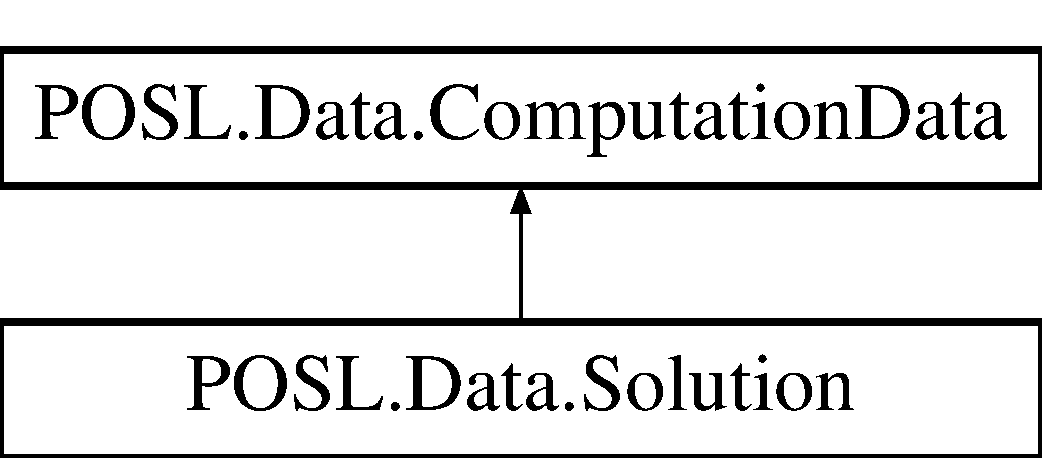
\includegraphics[height=2.000000cm]{classPOSL_1_1Data_1_1Solution}
\end{center}
\end{figure}
\subsection*{Public Member Functions}
\begin{DoxyCompactItemize}
\item 
\mbox{\Hypertarget{classPOSL_1_1Data_1_1Solution_a6f8f2ff8819270093192eef264fcb94a}\label{classPOSL_1_1Data_1_1Solution_a6f8f2ff8819270093192eef264fcb94a}} 
override string {\bfseries Tag} ()
\item 
\mbox{\Hypertarget{classPOSL_1_1Data_1_1Solution_a2a512552c56c237d0e763a42dd79023b}\label{classPOSL_1_1Data_1_1Solution_a2a512552c56c237d0e763a42dd79023b}} 
{\bfseries Solution} (\hyperlink{classPOSL_1_1Domain}{Domain} \+\_\+domains, int dimension)
\item 
\mbox{\Hypertarget{classPOSL_1_1Data_1_1Solution_ad41835bbe166b5a4d2f7e86ac225a488}\label{classPOSL_1_1Data_1_1Solution_ad41835bbe166b5a4d2f7e86ac225a488}} 
{\bfseries Solution} (\hyperlink{classPOSL_1_1Domain}{Domain} \+\_\+domains, int\mbox{[}$\,$\mbox{]} conf)
\item 
\mbox{\Hypertarget{classPOSL_1_1Data_1_1Solution_aafe2ae78ea574fd6441d66bc53d4f38f}\label{classPOSL_1_1Data_1_1Solution_aafe2ae78ea574fd6441d66bc53d4f38f}} 
\hyperlink{classPOSL_1_1Data_1_1Solution}{Solution} {\bfseries clone} ()
\item 
\mbox{\Hypertarget{classPOSL_1_1Data_1_1Solution_ae68f001d568db1822a965ccb8a8c6589}\label{classPOSL_1_1Data_1_1Solution_ae68f001d568db1822a965ccb8a8c6589}} 
void {\bfseries update\+Configuration} (int\mbox{[}$\,$\mbox{]} new\+\_\+config)
\item 
\mbox{\Hypertarget{classPOSL_1_1Data_1_1Solution_a10b51da92bbd9f24143dc89d1dbdb942}\label{classPOSL_1_1Data_1_1Solution_a10b51da92bbd9f24143dc89d1dbdb942}} 
void {\bfseries update\+Configuration\+From\+Pack} (int\mbox{[}$\,$\mbox{]} pack)
\item 
\mbox{\Hypertarget{classPOSL_1_1Data_1_1Solution_ad9de751fef1cd07ee4030f785b4d6c6f}\label{classPOSL_1_1Data_1_1Solution_ad9de751fef1cd07ee4030f785b4d6c6f}} 
override bool {\bfseries Equals} (object other)
\item 
\mbox{\Hypertarget{classPOSL_1_1Data_1_1Solution_a7d4ed9105296d47444202d6deb4a3686}\label{classPOSL_1_1Data_1_1Solution_a7d4ed9105296d47444202d6deb4a3686}} 
override int {\bfseries Get\+Hash\+Code} ()
\item 
\mbox{\Hypertarget{classPOSL_1_1Data_1_1Solution_a5ef760701c868dcdf65545fefeda89c7}\label{classPOSL_1_1Data_1_1Solution_a5ef760701c868dcdf65545fefeda89c7}} 
override string {\bfseries To\+String} ()
\item 
override int \hyperlink{classPOSL_1_1Data_1_1Solution_a17d810433104964cc43bf65f35d25cc7}{comapare\+To} (\hyperlink{classPOSL_1_1Data_1_1ComputationData}{Computation\+Data} other, Func$<$ \hyperlink{classPOSL_1_1Data_1_1ComputationData}{Computation\+Data}, int $>$ criteria)
\begin{DoxyCompactList}\small\item\em Compare this object with other, given a function (criteria) \end{DoxyCompactList}\end{DoxyCompactItemize}
\subsection*{Static Public Member Functions}
\begin{DoxyCompactItemize}
\item 
\mbox{\Hypertarget{classPOSL_1_1Data_1_1Solution_a62265e94c29382a7083fcc2c7d8a836f}\label{classPOSL_1_1Data_1_1Solution_a62265e94c29382a7083fcc2c7d8a836f}} 
static \hyperlink{structPOSL_1_1Tools_1_1T__Changes}{T\+\_\+\+Changes} {\bfseries get\+Changes} (int\mbox{[}$\,$\mbox{]} config\+\_\+before, \hyperlink{classPOSL_1_1Data_1_1Solution}{Solution} config\+\_\+after)
\end{DoxyCompactItemize}
\subsection*{Properties}
\begin{DoxyCompactItemize}
\item 
\mbox{\Hypertarget{classPOSL_1_1Data_1_1Solution_a5dde67410118890f2acb3e5d0d2cab68}\label{classPOSL_1_1Data_1_1Solution_a5dde67410118890f2acb3e5d0d2cab68}} 
int \mbox{[}$\,$\mbox{]} {\bfseries Get\+Conf\+By\+Copy}\hspace{0.3cm}{\ttfamily  \mbox{[}get\mbox{]}}
\item 
\mbox{\Hypertarget{classPOSL_1_1Data_1_1Solution_a7988dba5c7bd9ea33b52624474ee7f14}\label{classPOSL_1_1Data_1_1Solution_a7988dba5c7bd9ea33b52624474ee7f14}} 
int {\bfseries this\mbox{[}int index\mbox{]}}\hspace{0.3cm}{\ttfamily  \mbox{[}get, set\mbox{]}}
\item 
\mbox{\Hypertarget{classPOSL_1_1Data_1_1Solution_a88f278fd96c34ccda15720e2c6503d42}\label{classPOSL_1_1Data_1_1Solution_a88f278fd96c34ccda15720e2c6503d42}} 
int {\bfseries Length}\hspace{0.3cm}{\ttfamily  \mbox{[}get\mbox{]}}
\item 
\mbox{\Hypertarget{classPOSL_1_1Data_1_1Solution_acfa819580e4b046270604301c1ce47a1}\label{classPOSL_1_1Data_1_1Solution_acfa819580e4b046270604301c1ce47a1}} 
\hyperlink{classPOSL_1_1Domain}{Domain} {\bfseries Get\+Variables\+Domain}\hspace{0.3cm}{\ttfamily  \mbox{[}get\mbox{]}}
\item 
\mbox{\Hypertarget{classPOSL_1_1Data_1_1Solution_a870b7aba50a01904d1436f8e4b2f6226}\label{classPOSL_1_1Data_1_1Solution_a870b7aba50a01904d1436f8e4b2f6226}} 
string {\bfseries Solution\+Packing\+ID}\hspace{0.3cm}{\ttfamily  \mbox{[}get\mbox{]}}
\end{DoxyCompactItemize}


\subsection{Member Function Documentation}
\mbox{\Hypertarget{classPOSL_1_1Data_1_1Solution_a17d810433104964cc43bf65f35d25cc7}\label{classPOSL_1_1Data_1_1Solution_a17d810433104964cc43bf65f35d25cc7}} 
\index{P\+O\+S\+L\+::\+Data\+::\+Solution@{P\+O\+S\+L\+::\+Data\+::\+Solution}!comapare\+To@{comapare\+To}}
\index{comapare\+To@{comapare\+To}!P\+O\+S\+L\+::\+Data\+::\+Solution@{P\+O\+S\+L\+::\+Data\+::\+Solution}}
\subsubsection{\texorpdfstring{comapare\+To()}{comapareTo()}}
{\footnotesize\ttfamily override int P\+O\+S\+L.\+Data.\+Solution.\+comapare\+To (\begin{DoxyParamCaption}\item[{\hyperlink{classPOSL_1_1Data_1_1ComputationData}{Computation\+Data}}]{other,  }\item[{Func$<$ \hyperlink{classPOSL_1_1Data_1_1ComputationData}{Computation\+Data}, int $>$}]{criteria }\end{DoxyParamCaption})\hspace{0.3cm}{\ttfamily [inline]}, {\ttfamily [virtual]}}



Compare this object with other, given a function (criteria) 


\begin{DoxyParams}{Parameters}
{\em other} & The \hyperlink{classPOSL_1_1Data_1_1ComputationData}{Computation\+Data} to compare with. \\
\hline
{\em criteria} & A function (criteria). \\
\hline
\end{DoxyParams}
\begin{DoxyReturn}{Returns}
-\/1 if T\+H\+IS is lower, 1 if T\+H\+IS is bigger, 0 if equals 
\end{DoxyReturn}


Implements \hyperlink{classPOSL_1_1Data_1_1ComputationData_a6cca889bb4ce32104d91dba413ef8c56}{P\+O\+S\+L.\+Data.\+Computation\+Data}.



The documentation for this class was generated from the following file\+:\begin{DoxyCompactItemize}
\item 
P\+O\+S\+L/\+P\+O\+S\+L/\+Data/Solution.\+cs\end{DoxyCompactItemize}

\hypertarget{structPOSL_1_1Tools_1_1T__Changes}{}\section{P\+O\+S\+L.\+Tools.\+T\+\_\+\+Changes Struct Reference}
\label{structPOSL_1_1Tools_1_1T__Changes}\index{P\+O\+S\+L.\+Tools.\+T\+\_\+\+Changes@{P\+O\+S\+L.\+Tools.\+T\+\_\+\+Changes}}
\subsection*{Public Member Functions}
\begin{DoxyCompactItemize}
\item 
\mbox{\Hypertarget{structPOSL_1_1Tools_1_1T__Changes_a9962d6f4b60b953ea20d0ead8cadb616}\label{structPOSL_1_1Tools_1_1T__Changes_a9962d6f4b60b953ea20d0ead8cadb616}} 
{\bfseries T\+\_\+\+Changes} (int\mbox{[}$\,$\mbox{]} positions, int\mbox{[}$\,$\mbox{]} new\+\_\+values)
\end{DoxyCompactItemize}
\subsection*{Properties}
\begin{DoxyCompactItemize}
\item 
\mbox{\Hypertarget{structPOSL_1_1Tools_1_1T__Changes_ae3c0d4cff9f5570dd9dd9f2d4ef7dfbe}\label{structPOSL_1_1Tools_1_1T__Changes_ae3c0d4cff9f5570dd9dd9f2d4ef7dfbe}} 
int \mbox{[}$\,$\mbox{]} {\bfseries Positions}\hspace{0.3cm}{\ttfamily  \mbox{[}get\mbox{]}}
\item 
\mbox{\Hypertarget{structPOSL_1_1Tools_1_1T__Changes_a5f0bb645a4dc8b5c5349f070d5428ee5}\label{structPOSL_1_1Tools_1_1T__Changes_a5f0bb645a4dc8b5c5349f070d5428ee5}} 
int \mbox{[}$\,$\mbox{]} {\bfseries New\+Values}\hspace{0.3cm}{\ttfamily  \mbox{[}get\mbox{]}}
\item 
\mbox{\Hypertarget{structPOSL_1_1Tools_1_1T__Changes_a148a47ae6df3f5cf7c432456b8681684}\label{structPOSL_1_1Tools_1_1T__Changes_a148a47ae6df3f5cf7c432456b8681684}} 
int {\bfseries Dimension}\hspace{0.3cm}{\ttfamily  \mbox{[}get\mbox{]}}
\end{DoxyCompactItemize}


The documentation for this struct was generated from the following file\+:\begin{DoxyCompactItemize}
\item 
P\+O\+S\+L/\+P\+O\+S\+L/\+Tools/T\+\_\+\+Change.\+cs\end{DoxyCompactItemize}

\hypertarget{classPOSL_1_1Data_1_1UniformDomain}{}\section{P\+O\+S\+L.\+Data.\+Uniform\+Domain Class Reference}
\label{classPOSL_1_1Data_1_1UniformDomain}\index{P\+O\+S\+L.\+Data.\+Uniform\+Domain@{P\+O\+S\+L.\+Data.\+Uniform\+Domain}}
Inheritance diagram for P\+O\+S\+L.\+Data.\+Uniform\+Domain\+:\begin{figure}[H]
\begin{center}
\leavevmode
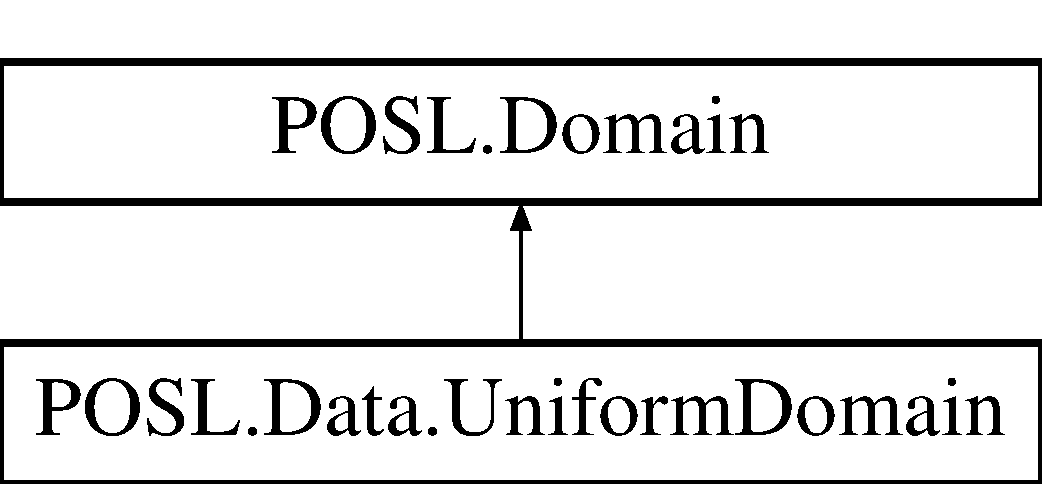
\includegraphics[height=2.000000cm]{classPOSL_1_1Data_1_1UniformDomain}
\end{center}
\end{figure}
\subsection*{Public Member Functions}
\begin{DoxyCompactItemize}
\item 
\mbox{\Hypertarget{classPOSL_1_1Data_1_1UniformDomain_acebfcc9bbe2917eb8f40a3170086e9a8}\label{classPOSL_1_1Data_1_1UniformDomain_acebfcc9bbe2917eb8f40a3170086e9a8}} 
{\bfseries Uniform\+Domain} (int \+\_\+min\+\_\+value, int \+\_\+max\+\_\+value)
\item 
\mbox{\Hypertarget{classPOSL_1_1Data_1_1UniformDomain_a0780e19ae2917dbea546cf6517e1c8b7}\label{classPOSL_1_1Data_1_1UniformDomain_a0780e19ae2917dbea546cf6517e1c8b7}} 
override int \mbox{[}$\,$\mbox{]} {\bfseries Get\+Values} (int variable)
\item 
\mbox{\Hypertarget{classPOSL_1_1Data_1_1UniformDomain_acb7a5863ffe580325f012dc04634e42d}\label{classPOSL_1_1Data_1_1UniformDomain_acb7a5863ffe580325f012dc04634e42d}} 
override int {\bfseries minimum} (int variable)
\item 
\mbox{\Hypertarget{classPOSL_1_1Data_1_1UniformDomain_a2e7e493c9fc263247405ae1337cf60ae}\label{classPOSL_1_1Data_1_1UniformDomain_a2e7e493c9fc263247405ae1337cf60ae}} 
override int {\bfseries maximum} (int variable)
\end{DoxyCompactItemize}


The documentation for this class was generated from the following file\+:\begin{DoxyCompactItemize}
\item 
P\+O\+S\+L/\+P\+O\+S\+L/\+Data/Uniform\+Domain.\+cs\end{DoxyCompactItemize}

%--- End generated contents ---

% Index
\backmatter
\newpage
\phantomsection
\clearemptydoublepage
\addcontentsline{toc}{chapter}{Index}
\printindex

\end{document}
